\documentclass[12pt,letterpaper]{article}
\usepackage{amsmath}
\usepackage{gensymb}
\usepackage[inline]{enumitem}
\usepackage{graphicx}
\usepackage[margin=1in]{geometry}
\setlength{\parindent}{0pt}
\title{Physics Club Practice Test 3}
\usepackage[export]{adjustbox}
\usepackage[none]{hyphenat}
\usepackage{titlesec}
\titlespacing{\section}{0pt}{4.0ex plus .2ex}{-3.3ex}
\titlespacing{\paragraph}{0pt}{0pt}{1em}
% \setenumerate[2]{label={\alph*.}}
\usepackage{fancyhdr}
\fancypagestyle{firstpage}
{
	\renewcommand{\headrulewidth}{0pt}
	\renewcommand{\footrulewidth}{0.4pt}
	\lfoot{Physics Club}
	\cfoot{$F=ma$ Practice Test 3}
	\rfoot{\thepage}
}
\thispagestyle{firstpage}
\pagestyle{fancy}
\fancyhf{}
\renewcommand{\headrulewidth}{0pt}
\renewcommand{\footrulewidth}{0.4pt}
\lfoot{Physics Club}
\cfoot{$F=ma$ Practice Test 3}
\rfoot{\thepage}
\begin{document}
\section*{Physics Club: $F=ma$ Practice Test 3}\hfill Version 1.0
\vspace{-2.5pt}
\begin{center}
\textsc{25 Questions -- 75 Minutes}
\end{center}
\vspace{-5pt}
Assume the acceleration due to gravity near the surface of the Earth $g = 10$ m/s$^2$.
\smallskip

Correct answers will be awarded one point; incorrect answers will result in a deduction of 1/4 point. There is no penalty for leaving an answer blank.
\smallskip

You may use a scientific calculator. Its memory must be cleared of data and programs.

\hrulefill

\begin{enumerate}
\item
As shown in the figure, a force $F$ pushes on a block $M$ which is placed on an inclined plane. The block is at rest. The following statements describe the friction acting on the block by the inclined plane.

\begin{tabular}{l r}

\begin{minipage}{0.6\textwidth}
\begin{enumerate}[label=\Roman*.]
\item The friction may be upward along the plane.
\item The friction may be downward along the plane.
\item The friction may be zero.
\item The friction may be larger than $F$.
\end{enumerate}
\end{minipage} &
\begin{minipage}{0.3\textwidth}
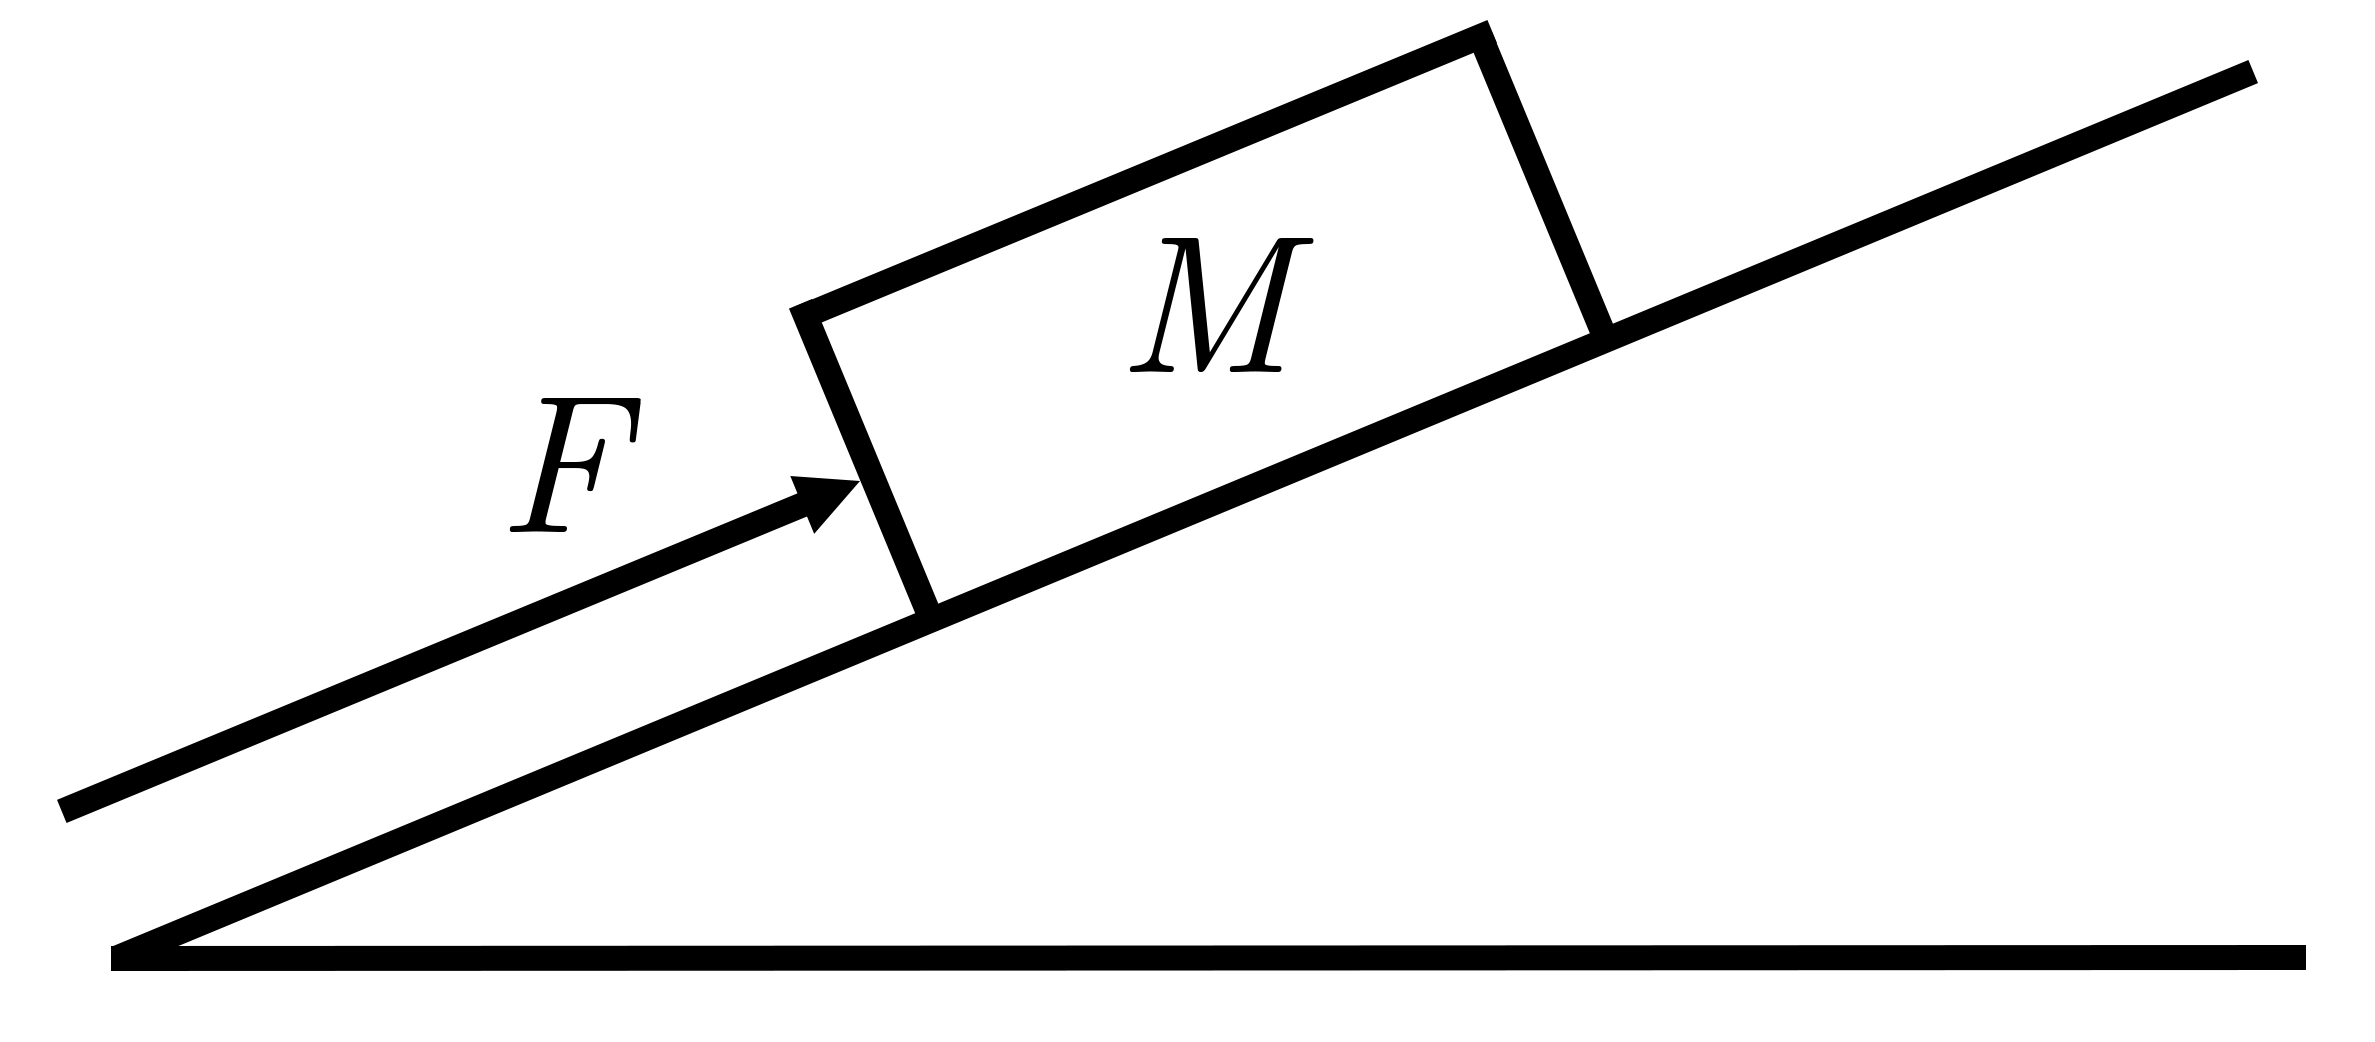
\includegraphics[width=\textwidth]{incline.png}
\end{minipage}
\end{tabular}

\begin{enumerate*}[itemjoin=\hfill]
\item I and II
\item I, II and III
\item II only
\item I only
\item I, II, III and IV
\end{enumerate*}

\item
An object is thrown with a fixed initial speed $v_0$ at various angles relative to the horizon. At some constant height $h$ above the launch point the speed $v$ of the object is measured as a function of the initial angle $\theta$. Which of the following best describes the dependence of $v$ on $\theta$? Assume that the height $h$ is achieved, and assume that there is no air resistance.
\begin{enumerate}
\item $v$ will increase monotonically with $\theta$.
\item $v$ will increase to some critical value $v_\text{max}$ and then decrease.
\item $v$ will remain constant, independent of $\theta$.
\item $v$ will decrease to some critical value $v_\text{min}$ and then increase.
\item None of the above.
\end{enumerate}

\item
An object of volume $V$ is submerged in a liquid of density $\rho$. It has a flat bottom of area $A$ which is at a depth of $H$ in the liquid, and a dome shaped top. Find the total force of liquid acting on the top of the object.

\begin{tabular}{l r}

\begin{minipage}{0.7\textwidth}
\begin{enumerate}
\item $\rho HAg-\rho Vg$ upward
\item $\rho HAg-\rho Vg$ downward
\item $\rho Vg$ upward
\item $\rho Vg$ downward
\item $\rho HAg$ upward
\end{enumerate}
\end{minipage} &
\begin{minipage}{0.2\textwidth}
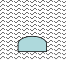
\includegraphics[width=\textwidth]{rock.png}
\end{minipage}
\end{tabular}

\item
An object is projected up an inclined plane with an initial speed of $v_0 = 10$ m/s, as shown in the diagram. The angle of the incline is $\theta = 30\degree$ above the horizontal direction and the coefficient of the sliding friction $\mu_k = 0.1$, the total time for the object to return to the point of projection is closest to

\begin{tabular}{l r}

\begin{minipage}{0.6\textwidth}
\begin{enumerate}
\item 3.81 s.
\item 4.26 s.
\item 4.54 s.
\item 4.94 s.
\item 5.32 s.
\end{enumerate}
\end{minipage} &
\begin{minipage}{0.3\textwidth}
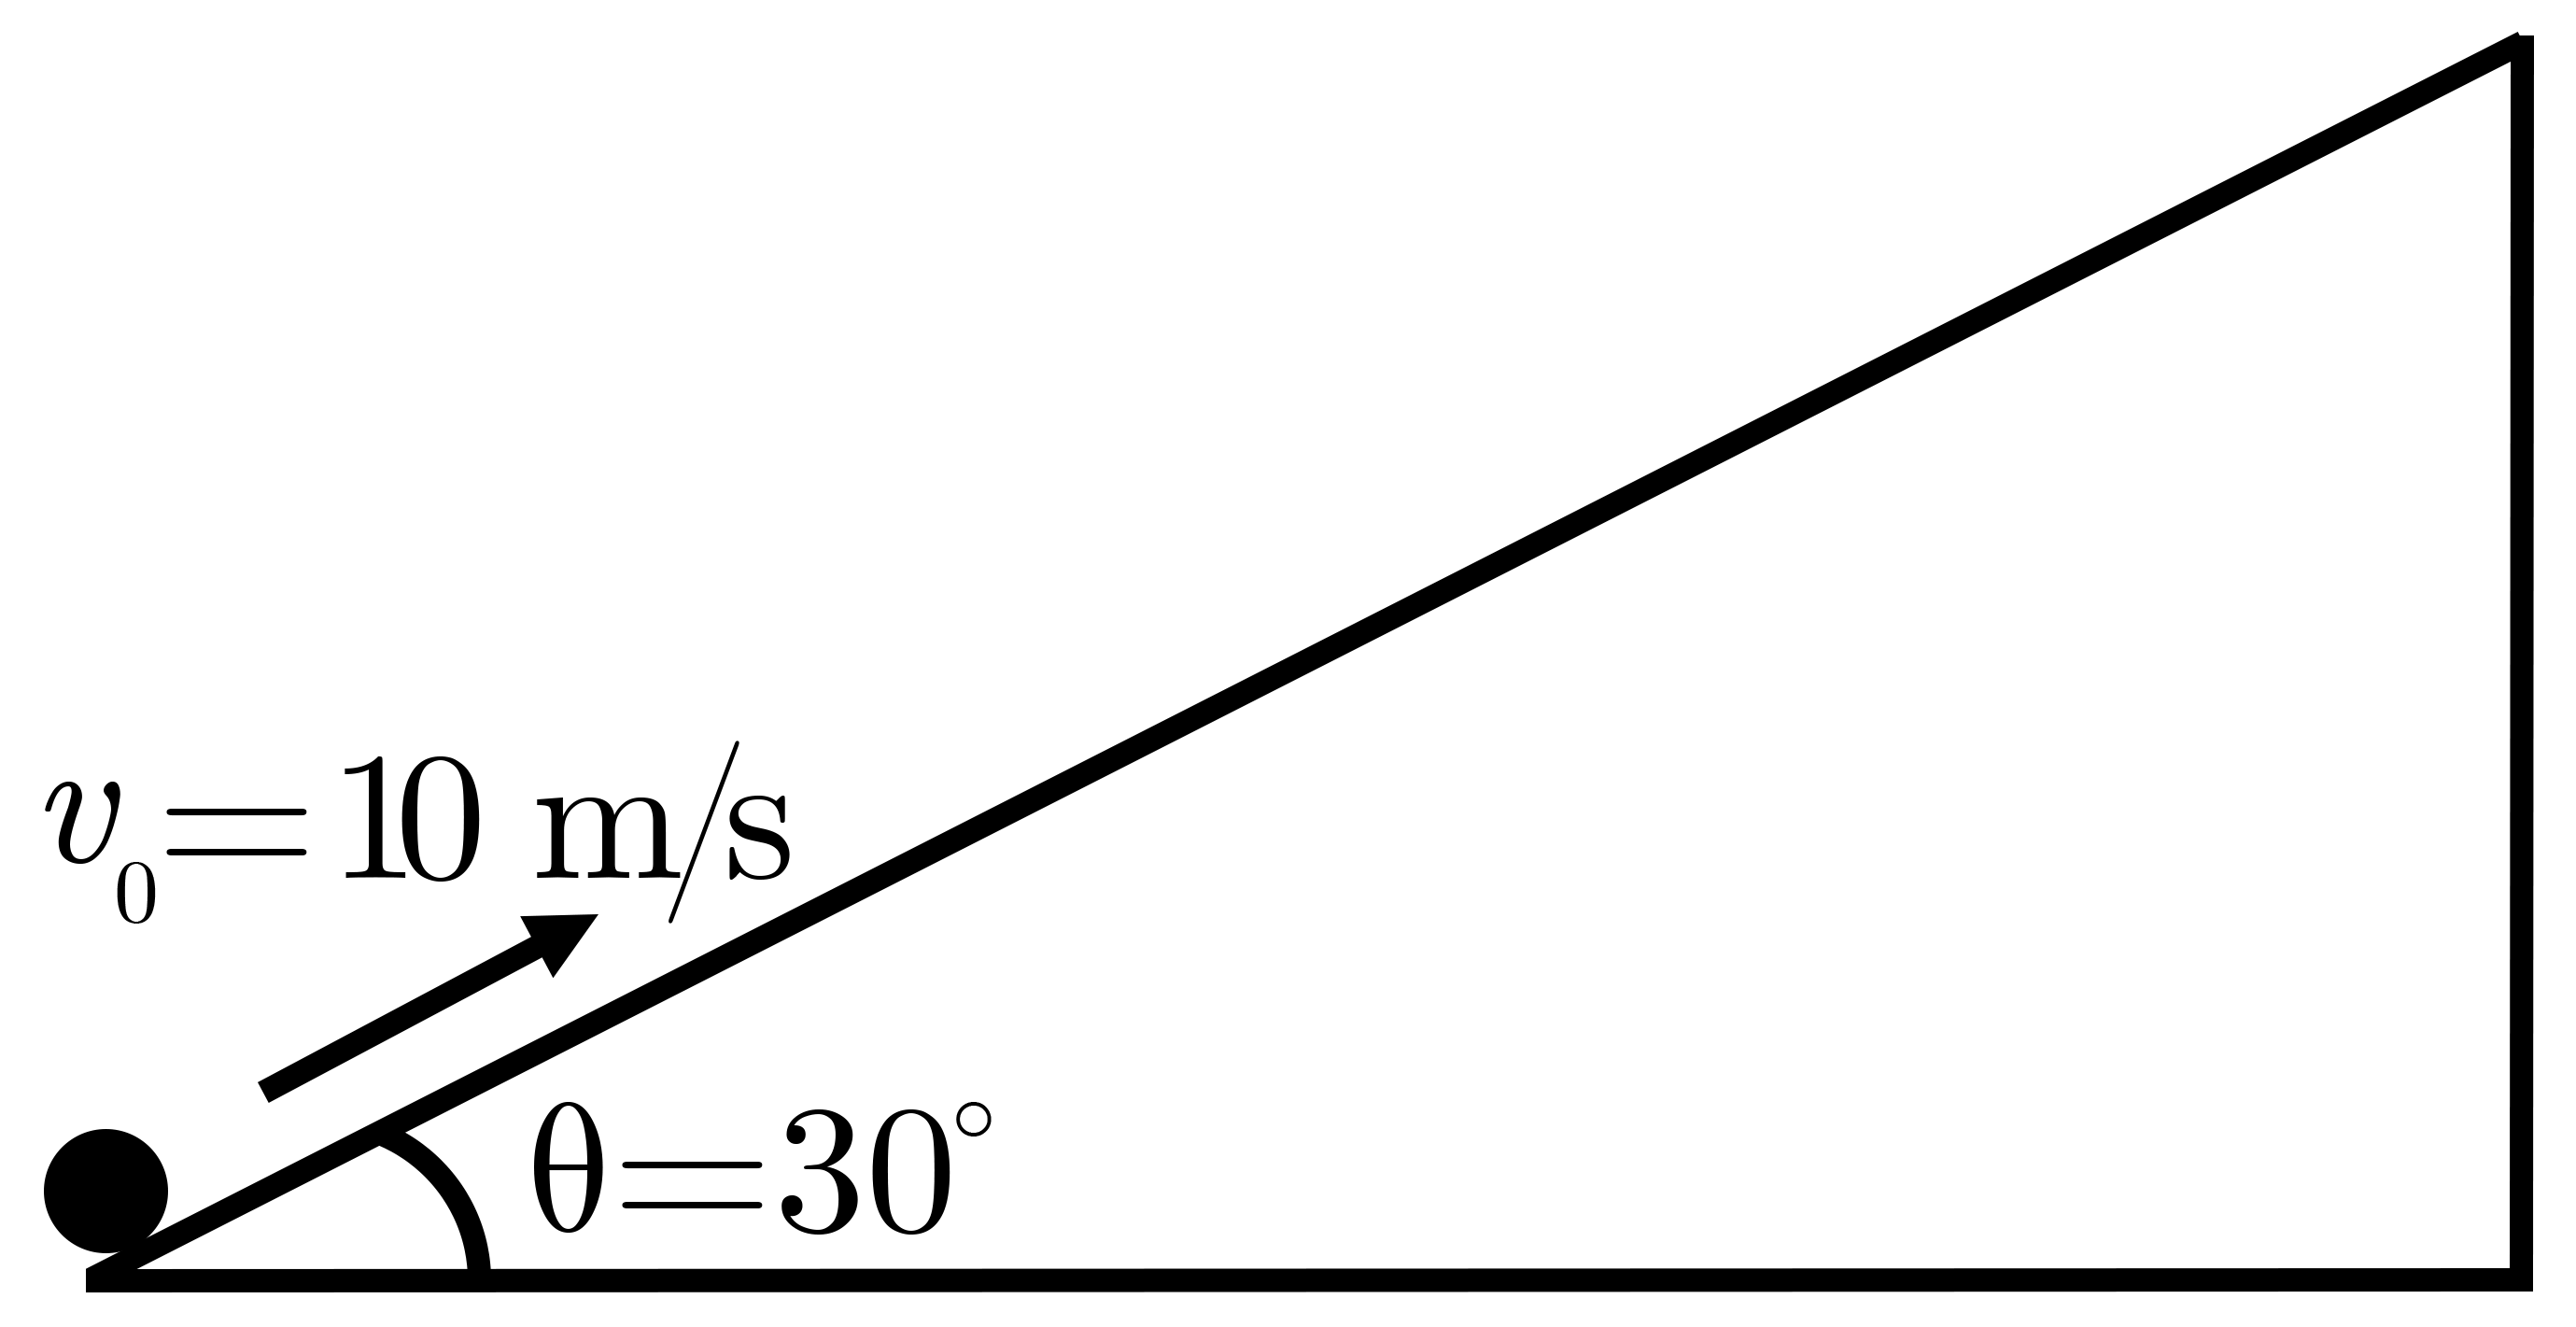
\includegraphics[width=\textwidth]{projection.png}
\end{minipage}
\end{tabular}
\end{enumerate}

\textbf{The following information is used for questions 5 and 6.}

\begin{tabular}{l r}

\begin{minipage}[t]{0.5\textwidth}
As shown in the figure, a boy is riding on a bus. The bus moves with a uniform speed of 20 km/h in a horizontal circle around the traffic light located at the center of the circle.
\end{minipage} &
\begin{minipage}[b]{0.5\textwidth}
\raisebox{\dimexpr-\height+\ht\strutbox\relax}{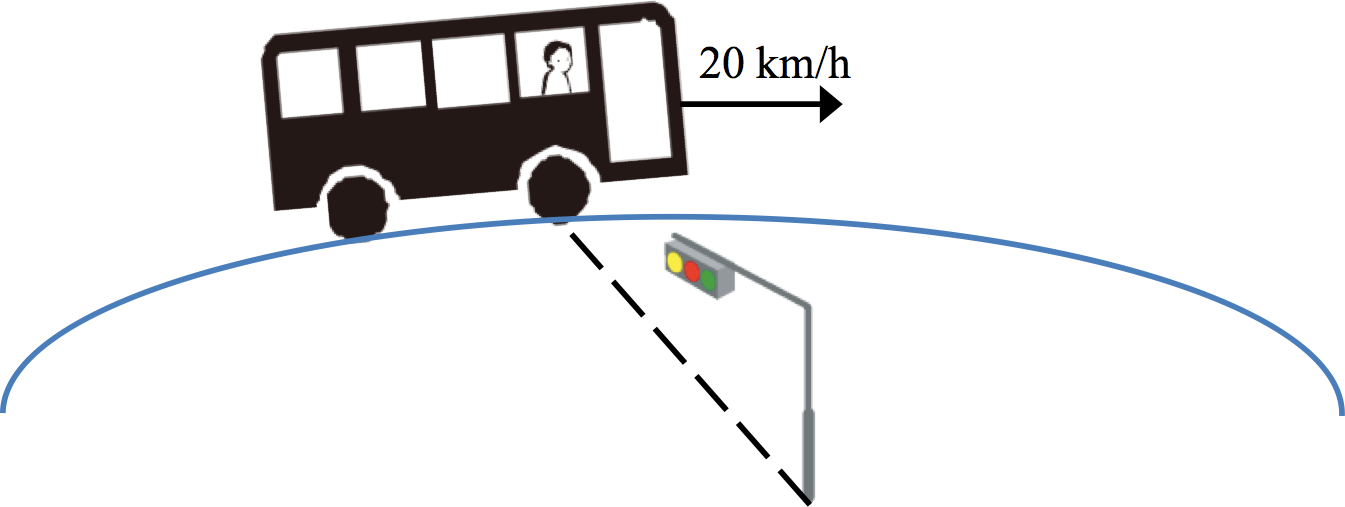
\includegraphics[width=\textwidth]{bus.png}}
\end{minipage}
\end{tabular}

\begin{enumerate}[resume]
\item
What is the velocity of the traffic light relative to the boy?
\begin{enumerate}
\item 20 km/h in the forward direction of the bus
\item 20 km/h in the backward direction of the bus
\item 20 km/h perpendicular to the forward direction of the bus and directed away from the bus
\item 20 km/h perpendicular to the forward direction of the bus and directed toward the bus
\item 0 km/h
\end{enumerate}

\item
A tennis ball machine is installed on the bus. It projects tennis balls at a speed of 100 km/h in the direction perpendicular to the forward direction of the bus, and on the outward side of the circular path. The trajectories of the tennis balls observed by the boy are
\begin{enumerate}
\item straight lines perpendicular to the forward direction of the bus.
\item straight lines slightly inclined toward the forward direction of the bus.
\item straight lines slightly inclined toward the backward direction of the bus.
\item curves slightly inclined toward the forward direction of the bus.
\item curves slightly inclined toward the backward direction of the bus.
\end{enumerate}

\item
A block of mass 0.50 kg is suspended form a spring balance and lowered into a beaker of water on a top pan balance as shown in the diagram below. If the mass of the beaker of water is 0.80 kg and the spring balance reads 3.0 N, what is the reading of the top pan balance?

\begin{tabular}{l r}

\begin{minipage}{0.5\textwidth}
\begin{enumerate}
\item 8.0 N
\item 9.0 N
\item 10.0 N
\item 11.0 N
\item 13.0 N
\end{enumerate}
\end{minipage} &
\begin{minipage}{0.4\textwidth}
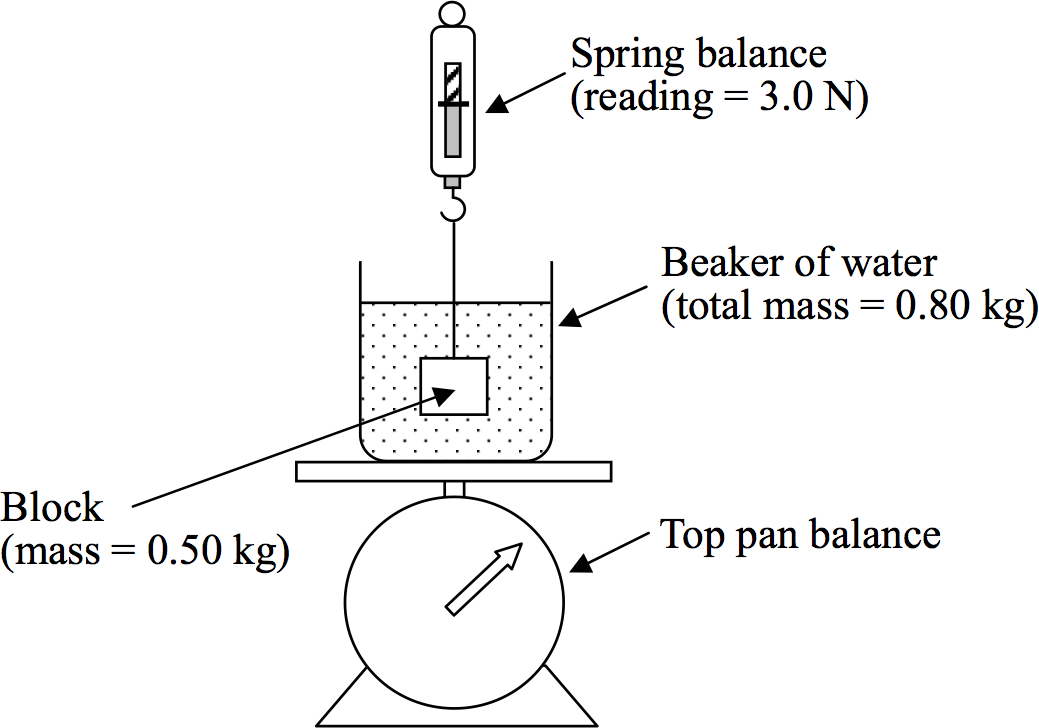
\includegraphics[width=\textwidth]{beaker.png}
\end{minipage}
\end{tabular}

\item
A man sits in the back of a canoe in still water. He then moves to the front of the canoe and sits there. Neglecting the damping of the water, the final position and the motion of the canoe are, respectively,
\begin{enumerate}
\item forward of its original position and moving forward.
\item forward of its original position and moving backward.
\item rearward of its original position and moving forward.
\item rearward of its original position and moving backward.
\item rearward of its original position and not moving.
\end{enumerate}

\item
In 1992 the first two extra-solar planets were discovered to be revolving around a pulsar of 1.5 solar masses. The period of the circular orbit of one of the two planets is 98 days. Ignore the gravitational interaction between the planets. Find the distance between the pulsar and the planet in terms of astronomical units (AU).
\begin{enumerate}
\item 0.11 AU
\item 0.17 AU
\item 0.36 AU
\item 0.40 AU
\item 0.48 AU
\end{enumerate}

\item
A sled loaded with children starts from rest and slides down a snowy $25\degree$ incline with respect to the horizontal traveling 85 meters in 17 seconds. Ignore air resistance. What is the coefficient of kinetic friction between the sled and the slope?
\begin{enumerate}
\item 0.31
\item 0.40
\item 0.53
\item 0.67
\item 0.73
\end{enumerate}

\vfill
\newpage

\item
A boat is about to cross a river to the opposite bank. The river water flows at a speed of 4 km/h. If the speed of the boat is 3 km/h, what should be the angle between the boat velocity and the upstream direction of the river, so that the downstream displacement is minimum when the boat reaches the opposite bank?
\begin{enumerate}
\item $0\degree$
\item $37\degree$
\item $41\degree$
\item $53\degree$
\item $90\degree$
\end{enumerate}

\item
It is given that the mass of Earth is $a$ times that of the Moon, and the radius of Earth is $b$ times that of the Moon. The period of a simple pendulum on Earth is $T$. When it is carried to the Moon, the period of the simple pendulum becomes
\begin{enumerate}
\item $\displaystyle T\frac{a}{\sqrt{b}}$
\item $\displaystyle T\frac{\sqrt{b}}{a}$
\item $\displaystyle T\frac{\sqrt{a}}{b}$
\item $\displaystyle T\frac{b}{\sqrt{a}}$
\item $\displaystyle T\sqrt{\frac{b}{a}}$
\end{enumerate}

\item
As shown in the figure, two wooden blocks A and B with masses $m_\text{A}$ and $m_\text{B}$ are placed on a smooth horizontal surface. When a horizontal force $F$ is acting on the left side of B, the accelerate together and the force between then is $N_1$. When a horizontal force $F$ is acting on the right side of A, the force between then is $N_2$. Determine which of the following statements are correct.

\begin{tabular}{l r}

\begin{minipage}{0.5\textwidth}
\begin{enumerate}[label=\Roman*.]
\item $N_1+N_2<F$
\item $N_1+N_2=F$
\item $N_1+N_2>F$
\item $\displaystyle \frac{N_1}{N_2}=\frac{m_\text{A}}{m_\text{B}}$
\end{enumerate}
\end{minipage} &
\begin{minipage}{0.4\textwidth}
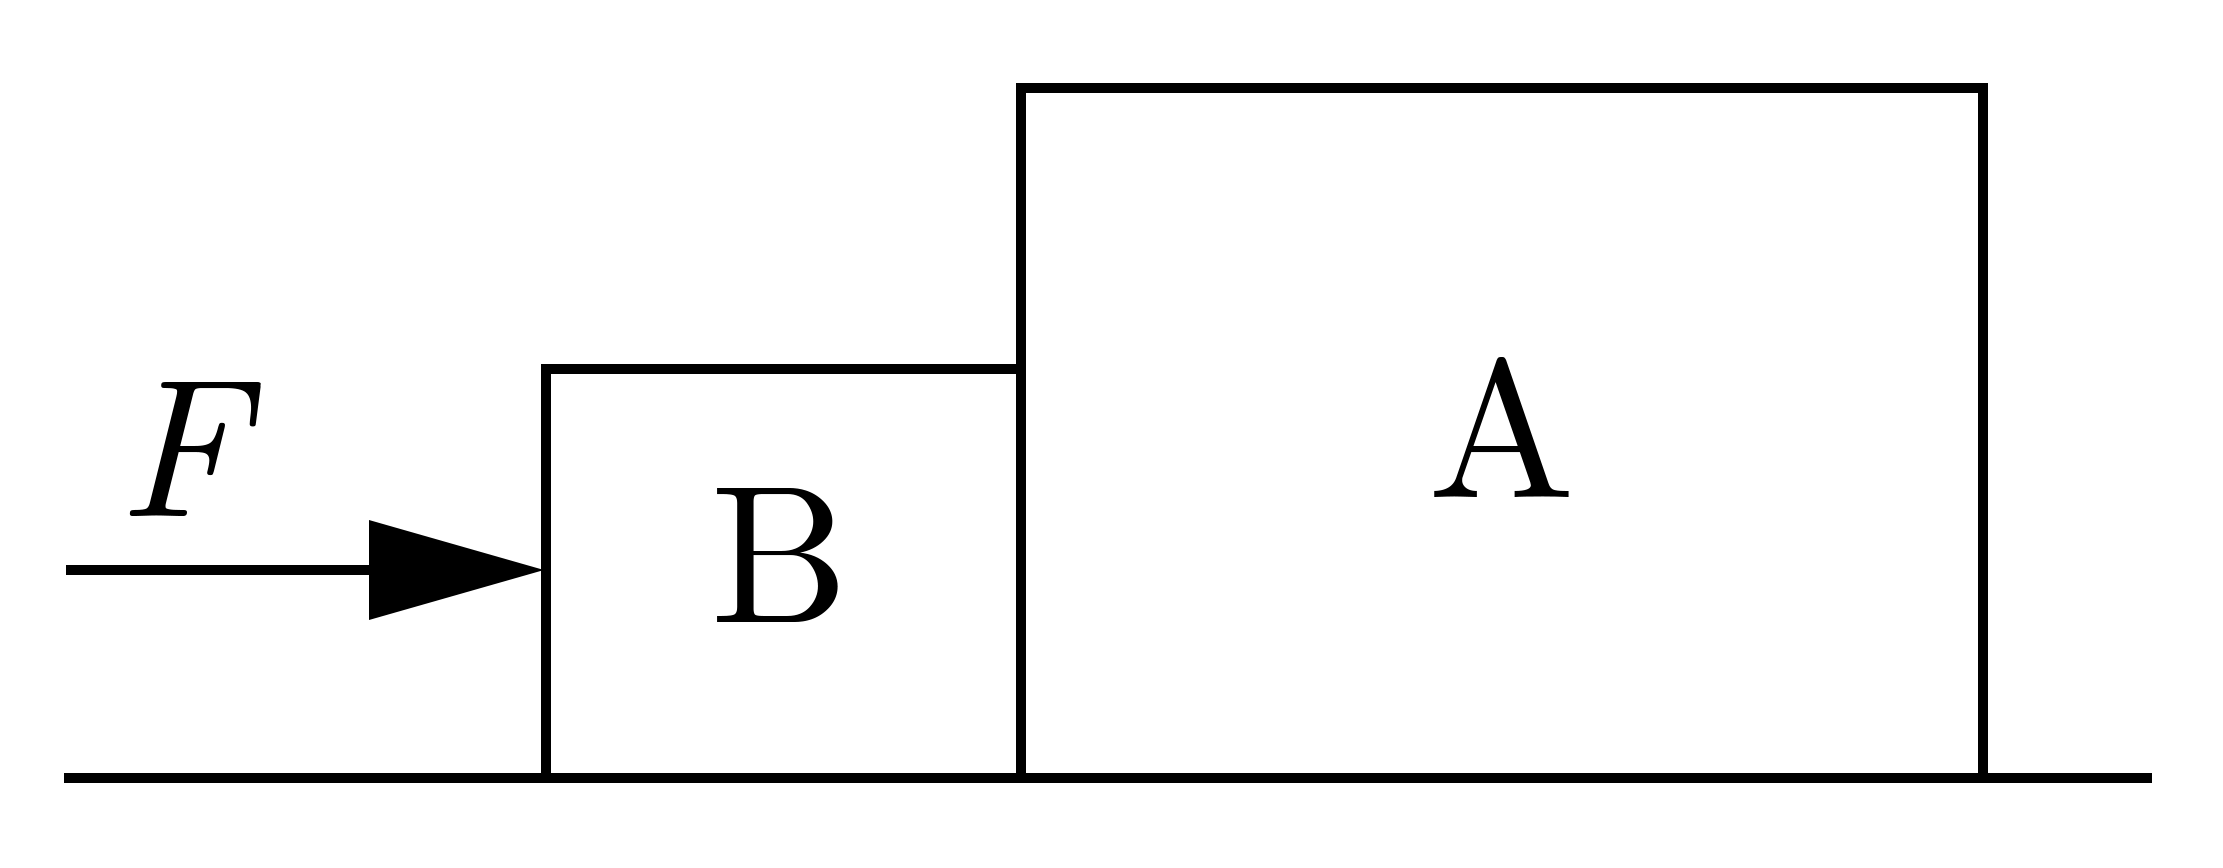
\includegraphics[width=\textwidth]{blocks.png}
\end{minipage}
\end{tabular}

\begin{enumerate*}[itemjoin=\hfill]
\item I and IV
\item II and IV
\item IV only
\item II only
\item III only
\end{enumerate*}

\vfill
\newpage

\item
As shown, four identical springs are placed horizontally on a force $F$ pulls at the right end of each of the springs. In diagram 1, the left end is attached to a wall. In diagram 2, the left end is acted by the same pulling force $F$. In diagram 3, the left end is attached to a small block which is placed on a smooth surface. In diagram 4, the left end is attached to a small block which is placed on a rough surface. Let $l_1$, $l_2$, $l_3$ and $l_4$ be the extensions of the four springs in diagrams 1, 2, 3 and 4, respectively. Neglect the masses of the springs, which of the following statements are correct?

\begin{tabular}{l r}

\begin{minipage}{0.2\textwidth}
\begin{enumerate}
\item $l_1<l_2$
\item $l_3<l_4$
\item $l_1>l_3$
\item $l_2=l_4$
\item $l_3>l_4$
\end{enumerate}
\end{minipage} &
\begin{minipage}{0.7\textwidth}
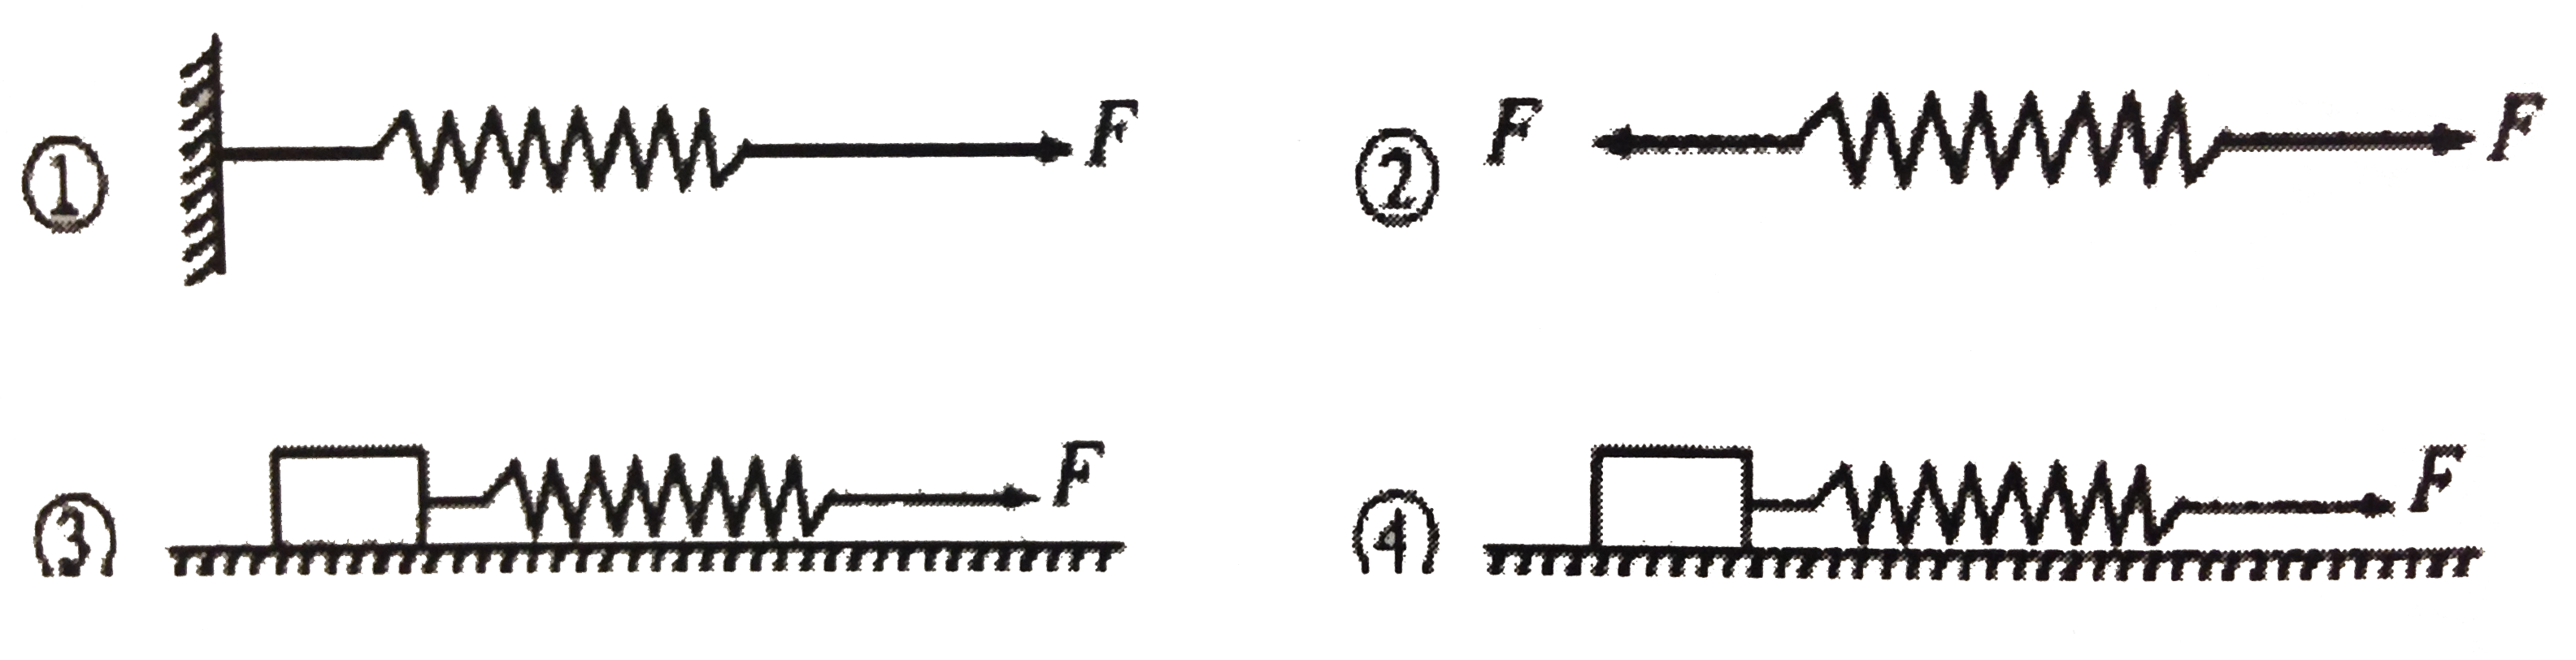
\includegraphics[width=\textwidth]{springs.png}
\end{minipage}
\end{tabular}

\item
As shown in the diagram, a light and soft thin wire is attached on the ceiling A and a vertical wall at B respectively. The points A and B are the same distance from point O. The length of the wire is twice of the distance between O and A. A mass $m$ is now hung on the wire with a smooth hook. The friction between the hook and the wire is negligible. What is the tension in the wire at equilibrium?

\begin{tabular}{l r}

\begin{minipage}{0.7\textwidth}
\begin{enumerate}
\item $mg$
\item $mg/\sqrt{2}$
\item $mg/2$
\item $mg/\sqrt{5}$
\item $mg/\sqrt{3}$
\end{enumerate}
\end{minipage} &
\begin{minipage}{0.2\textwidth}
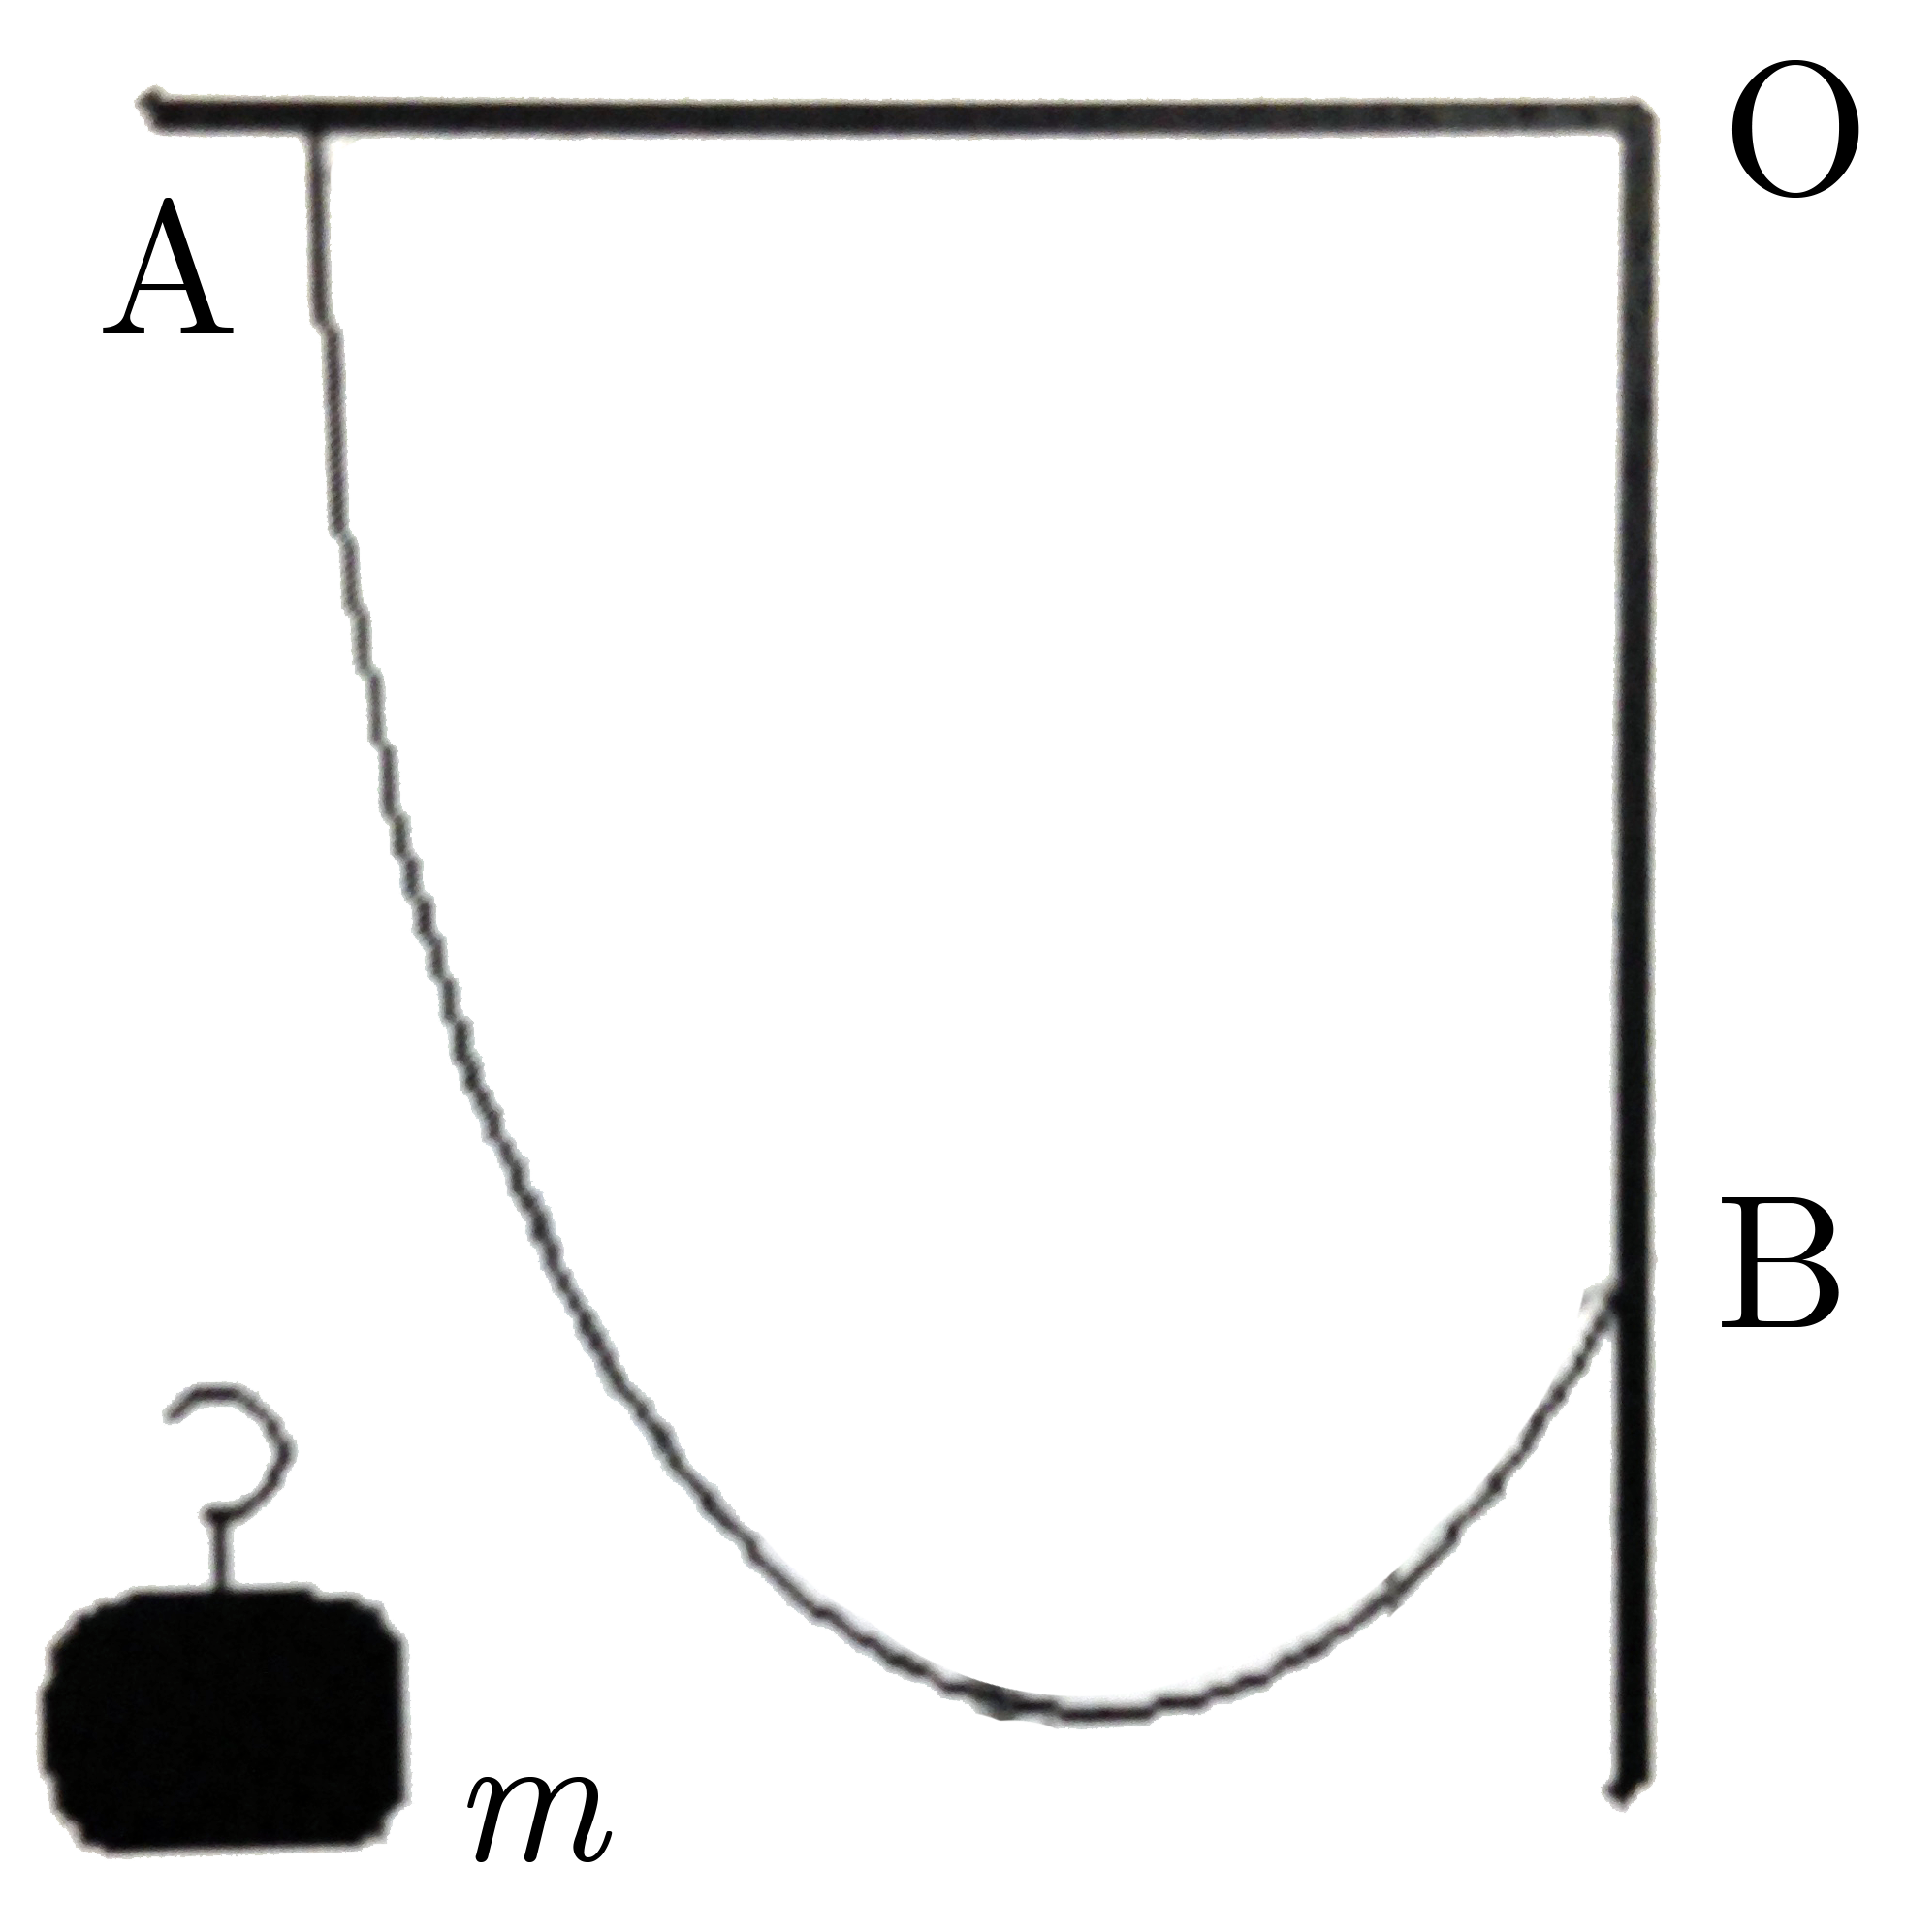
\includegraphics[width=\textwidth]{wire.png}
\end{minipage}
\end{tabular}

\item
Ignore friction between water and pipe wall. Water is pumped from a reservoir up to a height of 10 m at the rate of 30 kg/s through a pipe of $2.0 \times 10^{-3}$ m$^2$ in cross-sectional area. Find the pumping power.
\begin{enumerate}
\item 6315 W
\item 2940 W
\item 3573 W
\item 1305 W
\item 4960 W
\end{enumerate}

\vfill
\newpage

\item
As shown in the figure, a train with a length of $L = 500$ m moves by its inertia through the horizontal section of a railroad. However, the train encounters a small hill the slopes gently. With what minimum speed $v$ can the train cross the hill? The base of hill has a length $l = 100$ m, the lengths of the slopes of are $l_1 = 80$ m and $l_2 = 60$ m. The slopes of hill can be considered as straight lines and the small section of rounding at the top of the hill can be ignored. Neglect any friction.

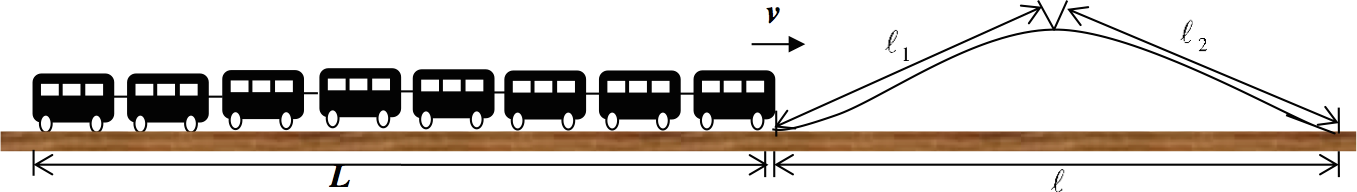
\includegraphics[width=0.9\textwidth]{train.png}
\begin{enumerate}
\item 9.6 m/s
\item 11.5 m/s
\item 13.2 m/s
\item 15.0 m/s
\item 16.2 m/s
\end{enumerate}

\item
There exist some triple star systems in the universe. They are more distant from other stars, and are composed of three stars of equal mass $M$. The gravitational forces due to other stars can be neglected. A basic stable structure of triple star systems consists of three collinear stars, with two companion stars moving around a central star on a circular orbit with radius $R$. The linear velocity of the companion stars is $v_1 = k\sqrt{GM/R}$, where $k$ is
\begin{enumerate}
\item $\sqrt{10}$.
\item $\sqrt{5}$.
\item $\sqrt{5/2}$.
\item $\sqrt{5}/2$.
\item $\sqrt[3]{5/2}$.
\end{enumerate}

\item
As shown in the diagram, the block-spring system is in equilibrium provided that the left spring is stretched by a displacement $x$. The whole system rests on a smooth supporting surface. The coefficient of static friction between the blocks is $\mu_s$, and the blocks have equal mass $m$. What is the maximum amplitude of the oscillations of the system such that the top block does not slide on the bottom one?

\begin{tabular}{l r}

\begin{minipage}{0.5\textwidth}
\begin{enumerate}
\item $\displaystyle \frac{\mu_s mg}{2k}+x$
\item $4kx-\mu_s mg$
\item $\displaystyle \frac{\mu_s mg}{k}-x$
\item $2(2kx+\mu_s mg)$
\item $2(2kx-\mu_s mg)$
\end{enumerate}
\end{minipage} &
\begin{minipage}{0.4\textwidth}
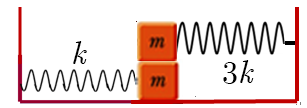
\includegraphics[width=\textwidth]{spring.png}
\end{minipage}
\end{tabular}

\vfill
\newpage

\item
As shown in the diagram, a small block of mass $m$ is released from rest at the top of a smooth track which is on a large block. The large block of mass $M$ is at rest on a smooth surface. The track forms a quarter of a circle with radius $R$. The small block slides from the top to the bottom of the track where the tangent is horizontal. Determine the work done by the normal force on the small block in th whole process.

\begin{tabular}{l r}

\begin{minipage}{0.6\textwidth}
\begin{enumerate}
\item $\displaystyle -\frac{m^2gR}{m+M}$
\item $\displaystyle \frac{mMgR}{m+M}$
\item $\displaystyle -\frac{mMgR}{m+M}$
\item $mgR$
\item 0
\end{enumerate}
\end{minipage} &
\begin{minipage}{0.3\textwidth}
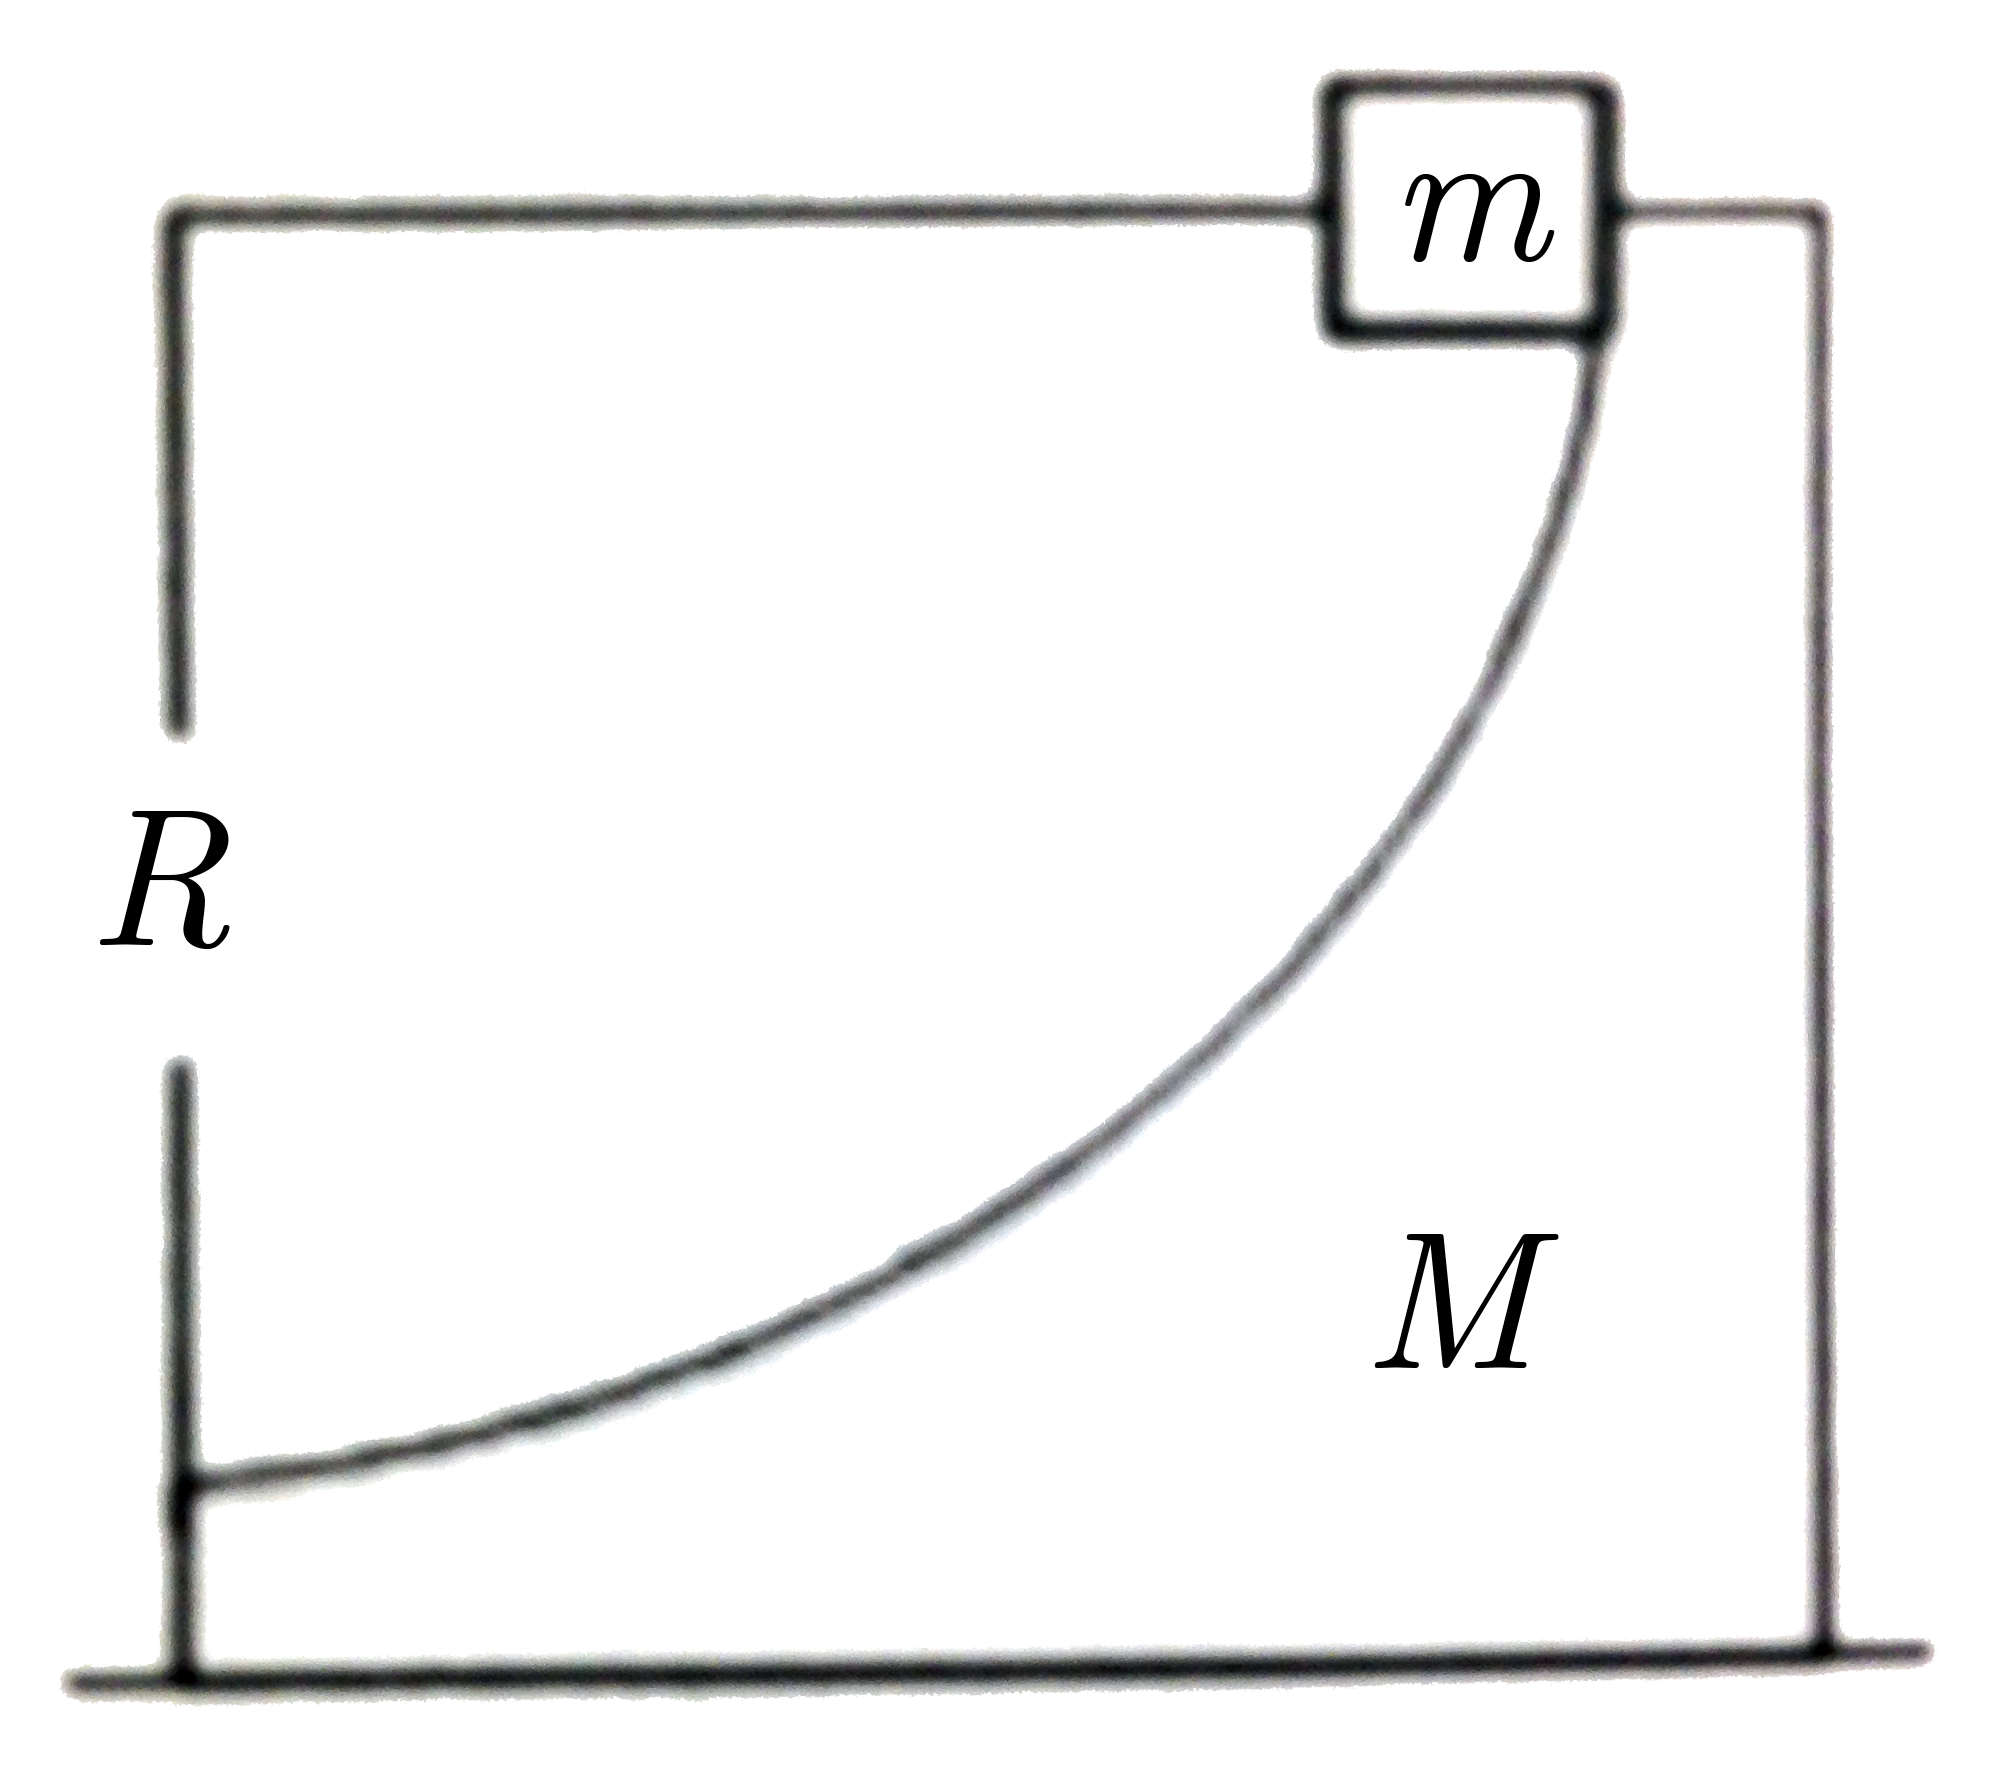
\includegraphics[width=\textwidth]{track.png}
\end{minipage}
\end{tabular}

\item
A U tube which is partially filled with liquid is in a vehicle that is accelerating horizontally with an acceleration $a > 0$, as shown in the diagram. Find the maximum difference in height of the liquid surface over the lateral distance of $L$.

\begin{tabular}{l r}

\begin{minipage}{0.7\textwidth}
\begin{enumerate}
\item $\displaystyle \frac{g}{a}L$
\item $\displaystyle \frac{a}{\sqrt{g^2+a^2}}L$
\item $\displaystyle \frac{a}{g}L$
\item $\displaystyle \sqrt\frac{a}{g}L$
\item $\displaystyle \frac{g}{\sqrt{g^2+a^2}}L$
\end{enumerate}
\end{minipage} &
\begin{minipage}{0.2\textwidth}
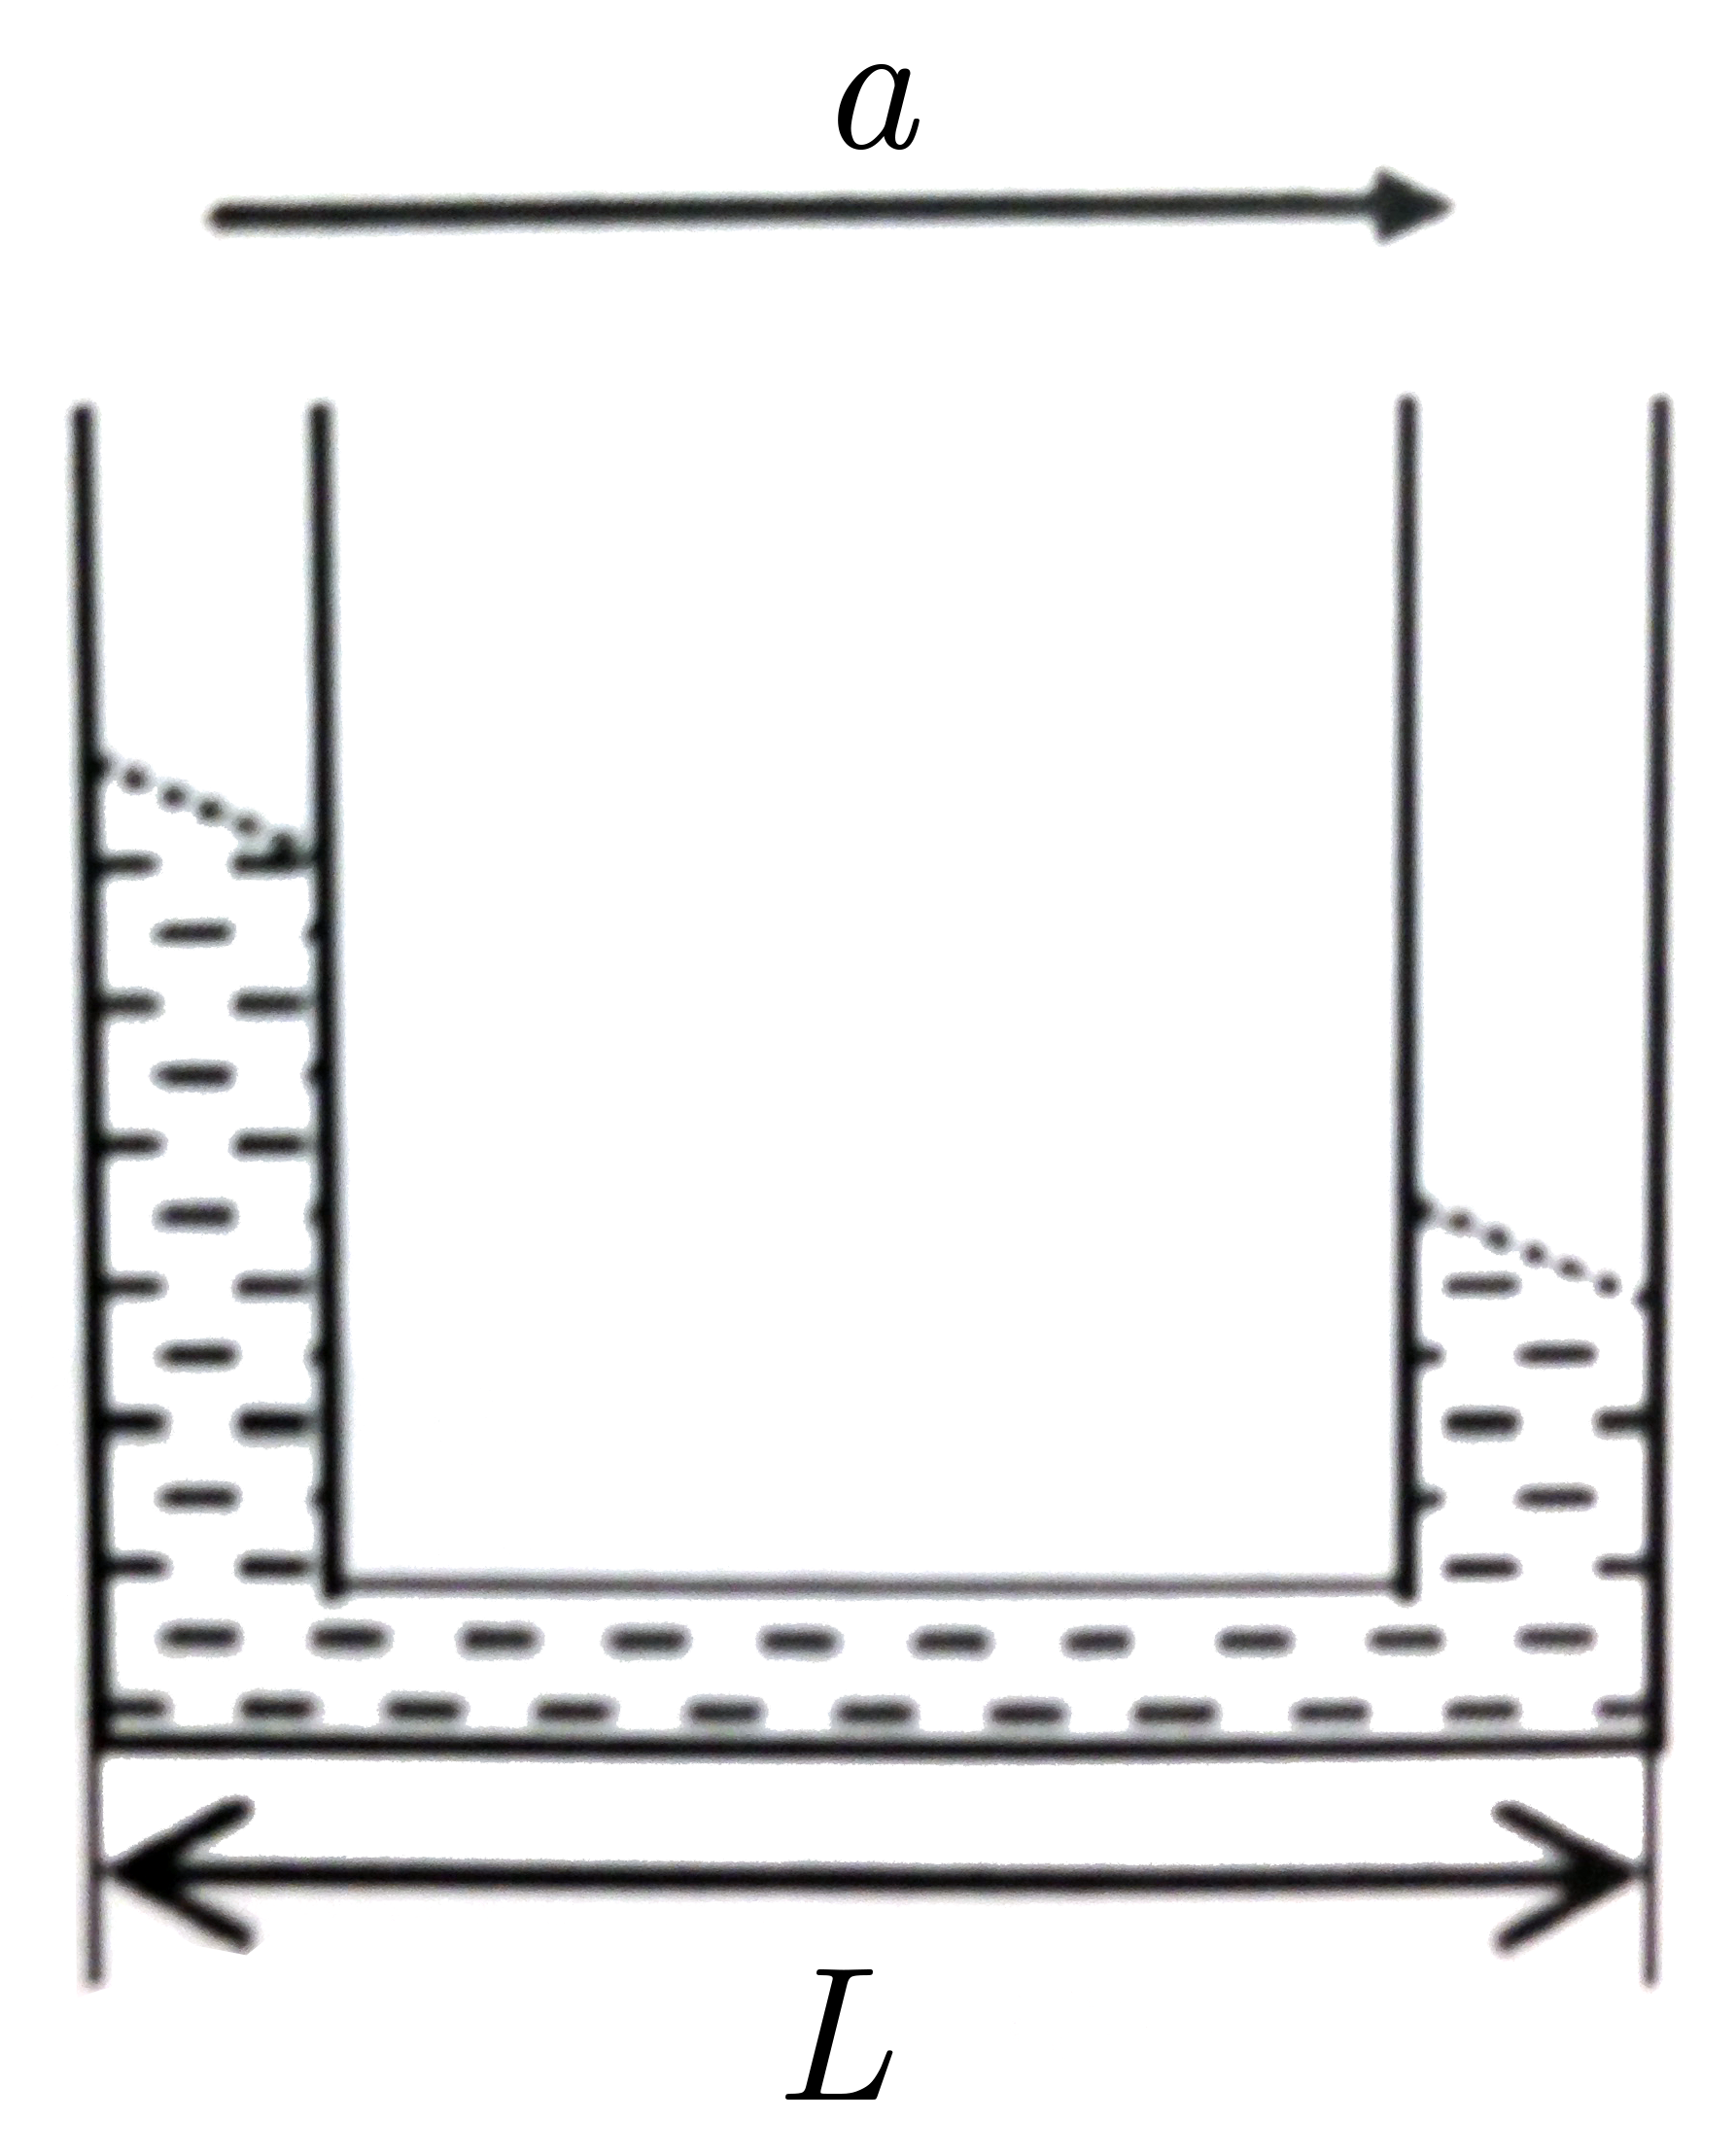
\includegraphics[width=\textwidth]{utube.png}
\end{minipage}
\end{tabular}

\item
On a plane inclined at a $30\degree$ angle, a wooden block of mass $m_2 = 4$ kg is connected with a solid cylinder of mass $m_1 = 8$ kg and radius $r = 5$ cm. The coefficient of kinetic friction between the wooden block and the inclined plane is $\mu = 0.2$. When the system is released, the wooden block slides and the cylinder rolls down the inclined plane without slipping. The acceleration of the system is closest to

\begin{tabular}{l r}

\begin{minipage}{0.6\textwidth}
\begin{enumerate}
\item 5.95 m/s$^2$
\item 5.12 m/s$^2$
\item 4.38 m/s$^2$
\item 3.92 m/s$^2$
\item 3.32 m/s$^2$
\end{enumerate}
\end{minipage} &
\begin{minipage}{0.3\textwidth}
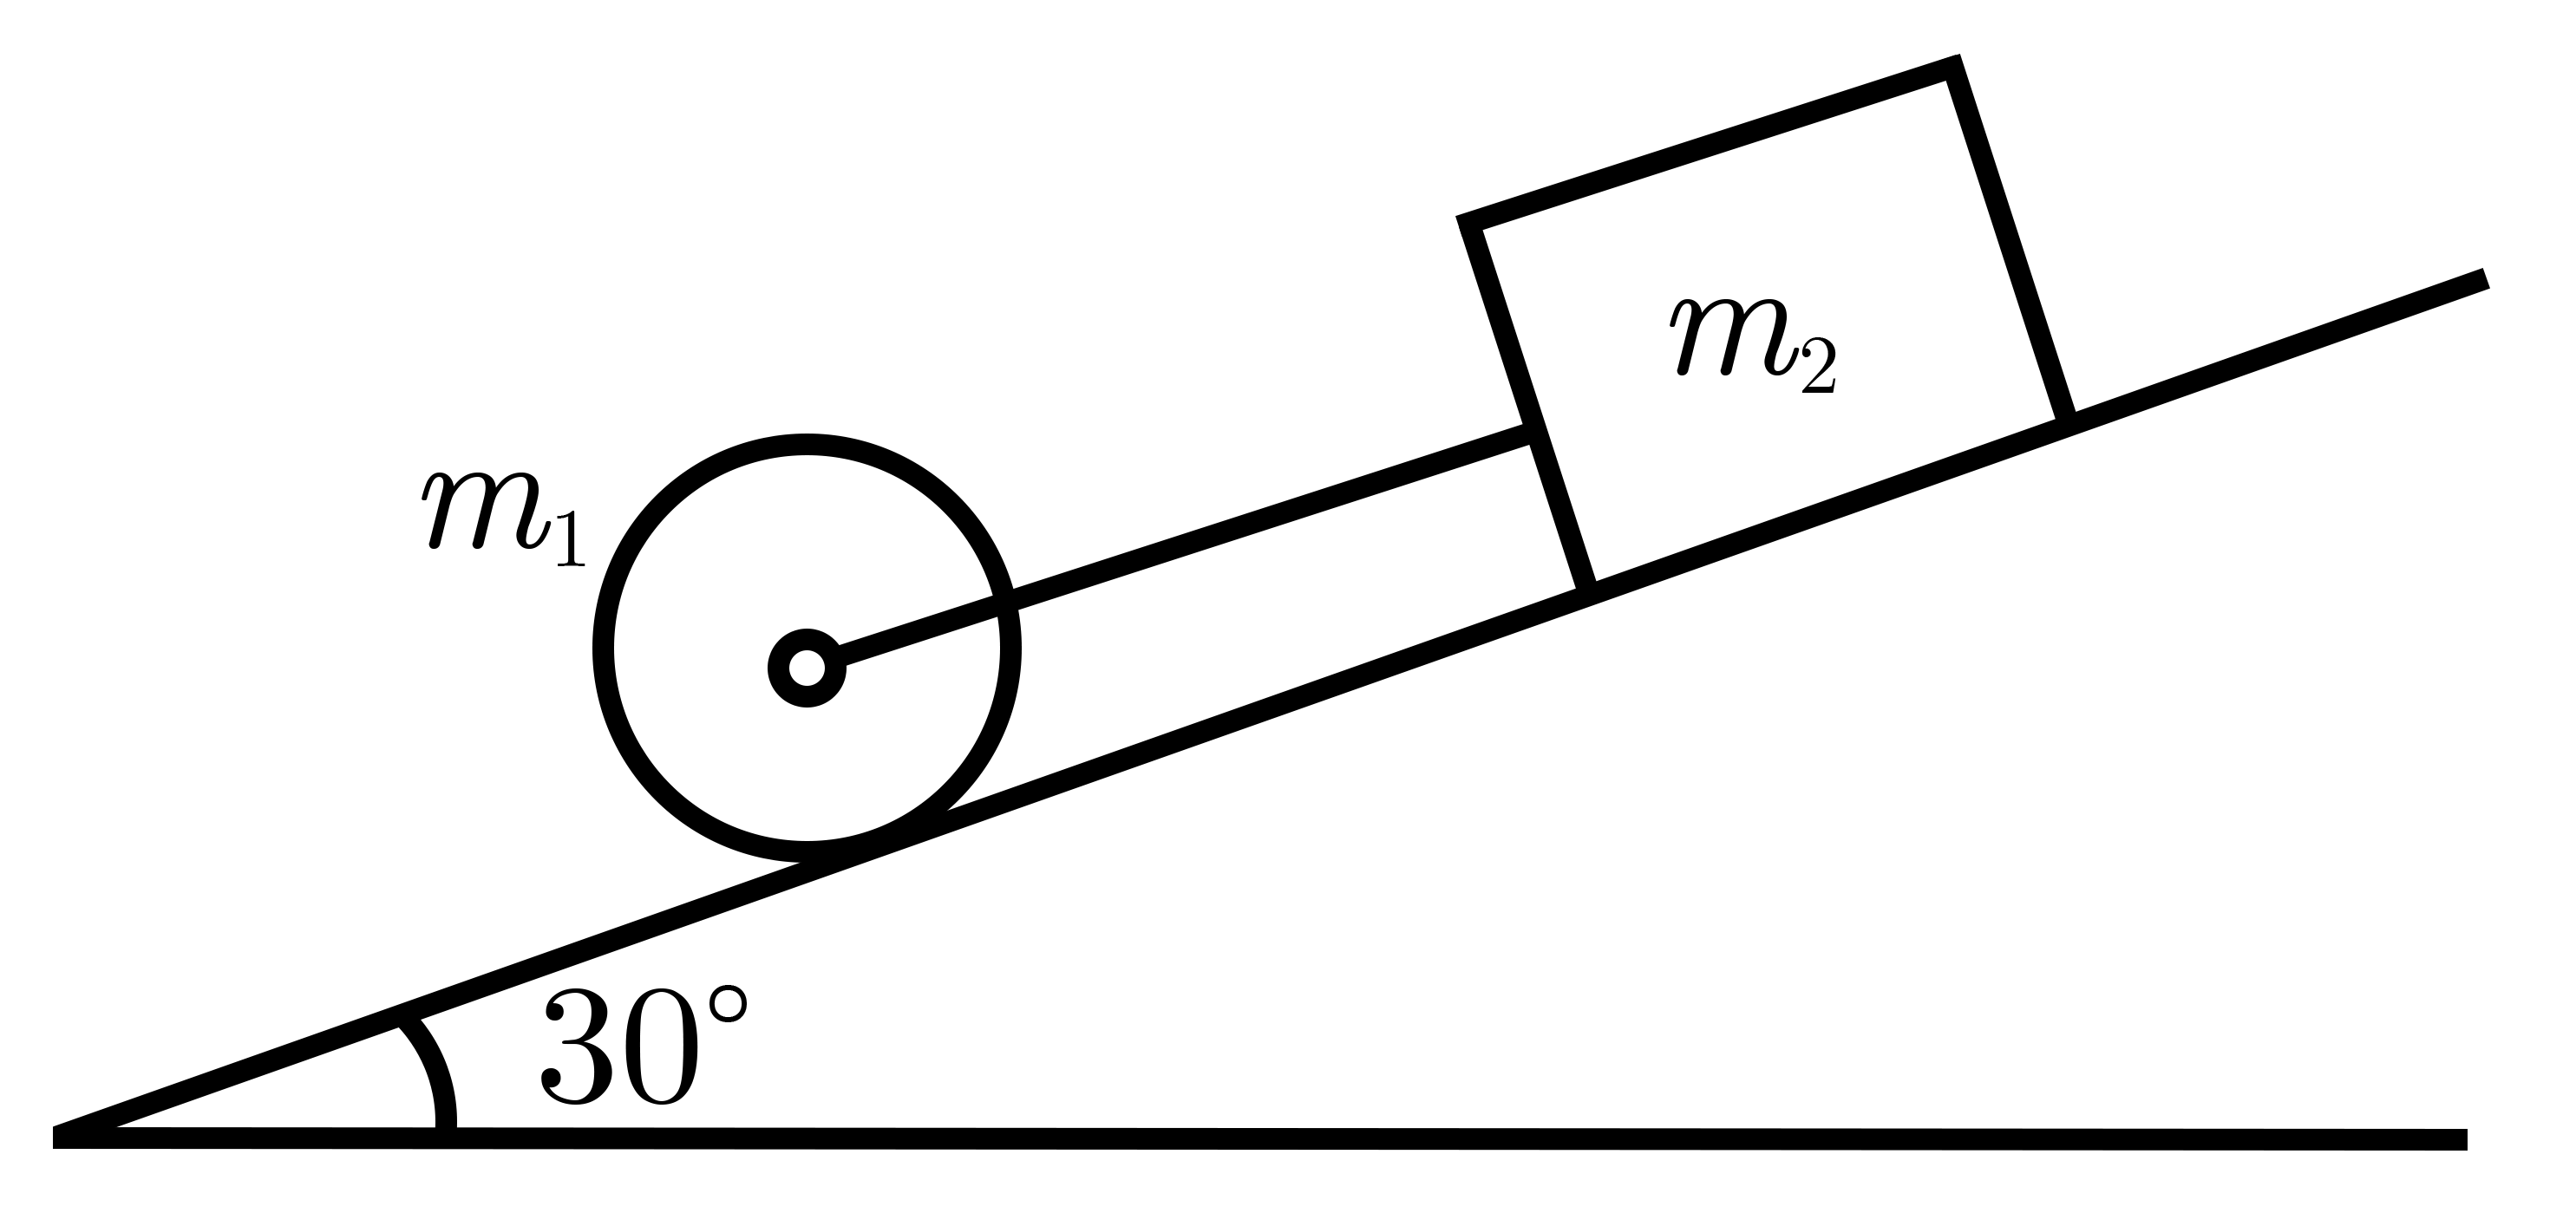
\includegraphics[width=\textwidth]{cylinder.png}
\end{minipage}
\end{tabular}

\item
The rebound coefficient between a tennis ball and a racket is defined as $\gamma = v_2/v_1$, where $v_1$ is the incoming speed of the ball and $v_2$ is the speed of the ball after rebound while the racket is at rest. A tennis ball falls from height $H$ to a racket at rest and bounces back to $0.8H$. A tennis player is using the racket to hit an incoming tennis ball traveling at 150 km/h and the racket is moving at 100 km/h. What is the speed of the ball after being hit? Assume the mass of the racket is much greater than that of the ball.
\begin{enumerate}
\item 324 km/h
\item 350 km/h
\item 150 km/h
\item 250 km/h
\item 234 km/h
\end{enumerate}

\item
Two small and hard spheres, one right on top of the other and almost in touch, are left to fall from a height $H$. The lower sphere of mass $M$ collides with the ground, and almost instantaneously it collides with the upper sphere of mass $m = M/10$. Both collisions are elastic. Find the maximum height the upper sphere can reach.

\begin{tabular}{l r}

\begin{minipage}{0.8\textwidth}
\begin{enumerate}
\item $6.95H$
\item $6.15H$
\item $5.56H$
\item $4.95H$
\item $4.05H$
\end{enumerate}
\end{minipage} &
\begin{minipage}{0.1\textwidth}
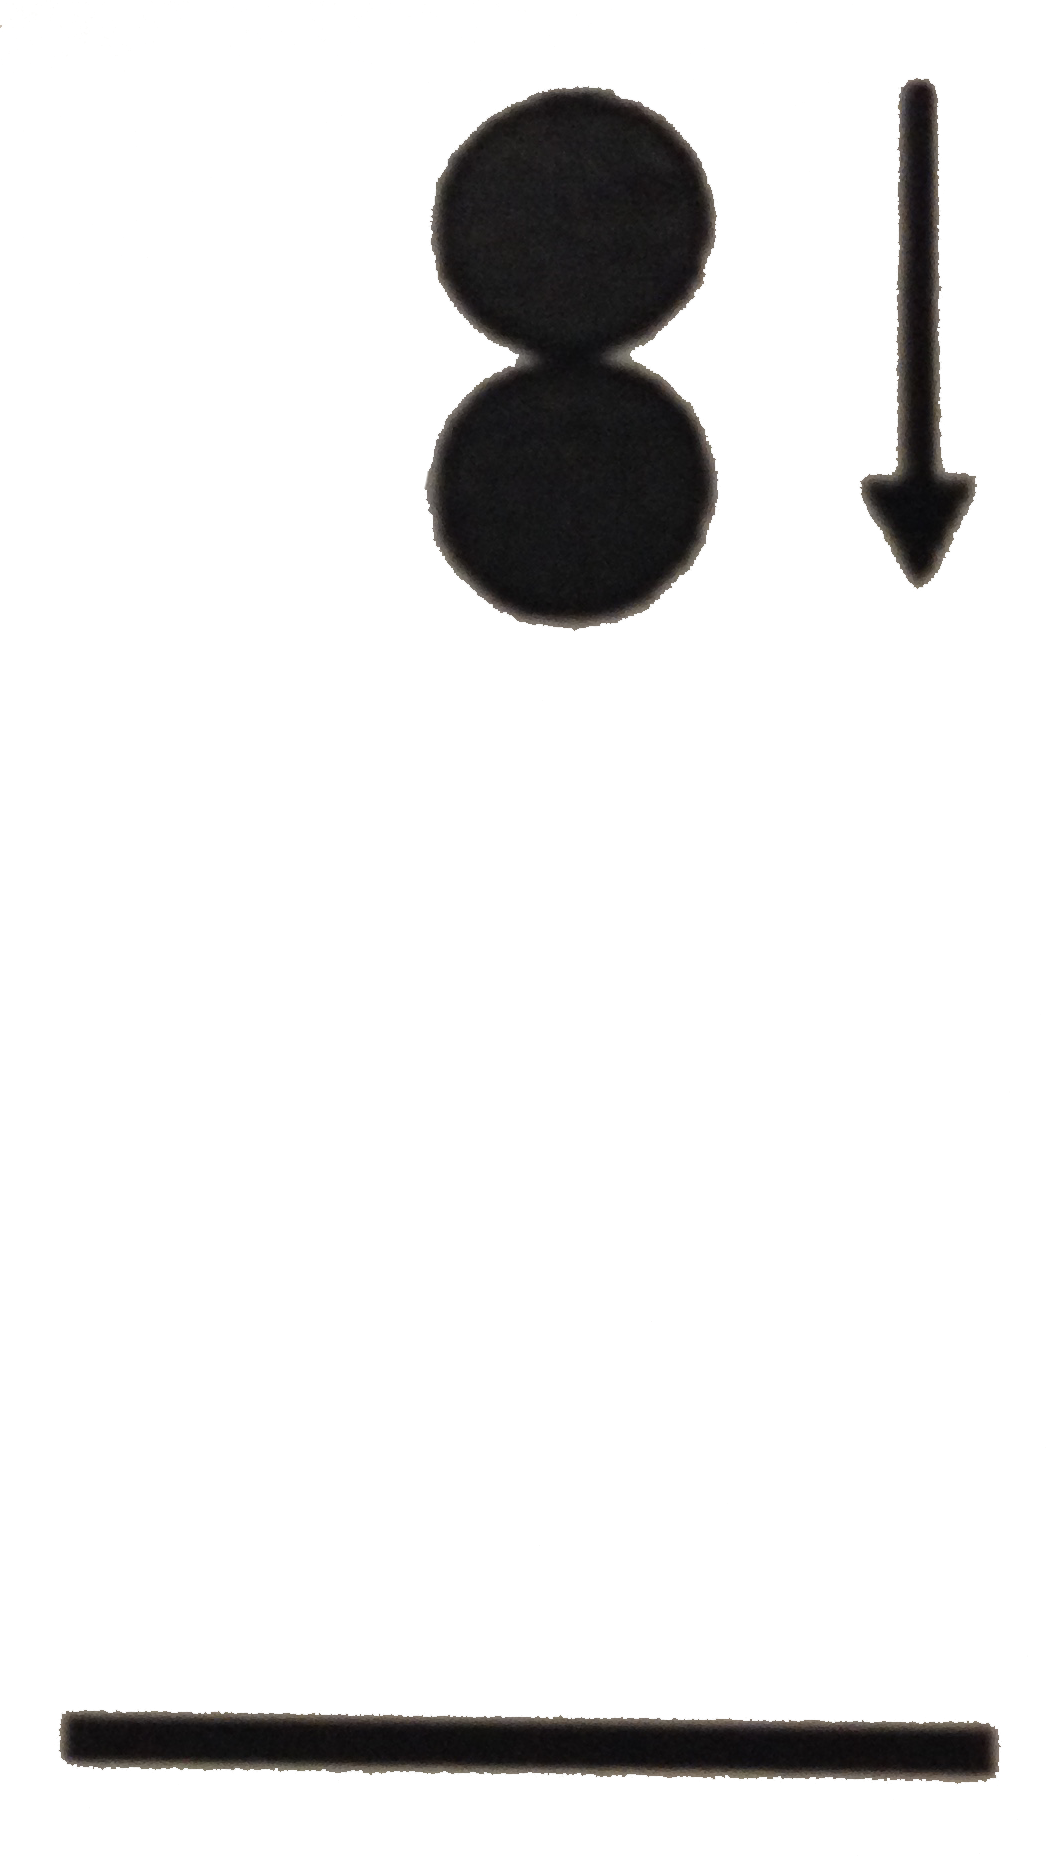
\includegraphics[width=\textwidth]{spheres.png}
\end{minipage}
\end{tabular}

\item
A small block A of mass $m$ resting on a smooth horizontal plane is attached by threads to a point P and, by means of a massless pulley, to a block B of the same mass $m$. Besides, block A is also attached to a point O by means of a light unstretched spring of length $l_0$ and spring constant $k=5mg/l_0$ where $g$ is the acceleration of gravity. Block A starts moving when the thread PA is burned. Find the velocity of block A at the moment when it is breaking off the plane.

\begin{tabular}{l r}

\begin{minipage}{0.6\textwidth}
\begin{enumerate}
\item $\displaystyle \sqrt{\frac{3}{8}gl_0}$
\item $\displaystyle \frac{1}{2}\sqrt{gl_0}$
\item $\displaystyle \sqrt{\frac{13}{32}gl_0}$
\item $\displaystyle \sqrt{\frac{19}{32}gl_0}$
\item $\sqrt{gl_0}$
\end{enumerate}
\end{minipage} &
\begin{minipage}{0.3\textwidth}
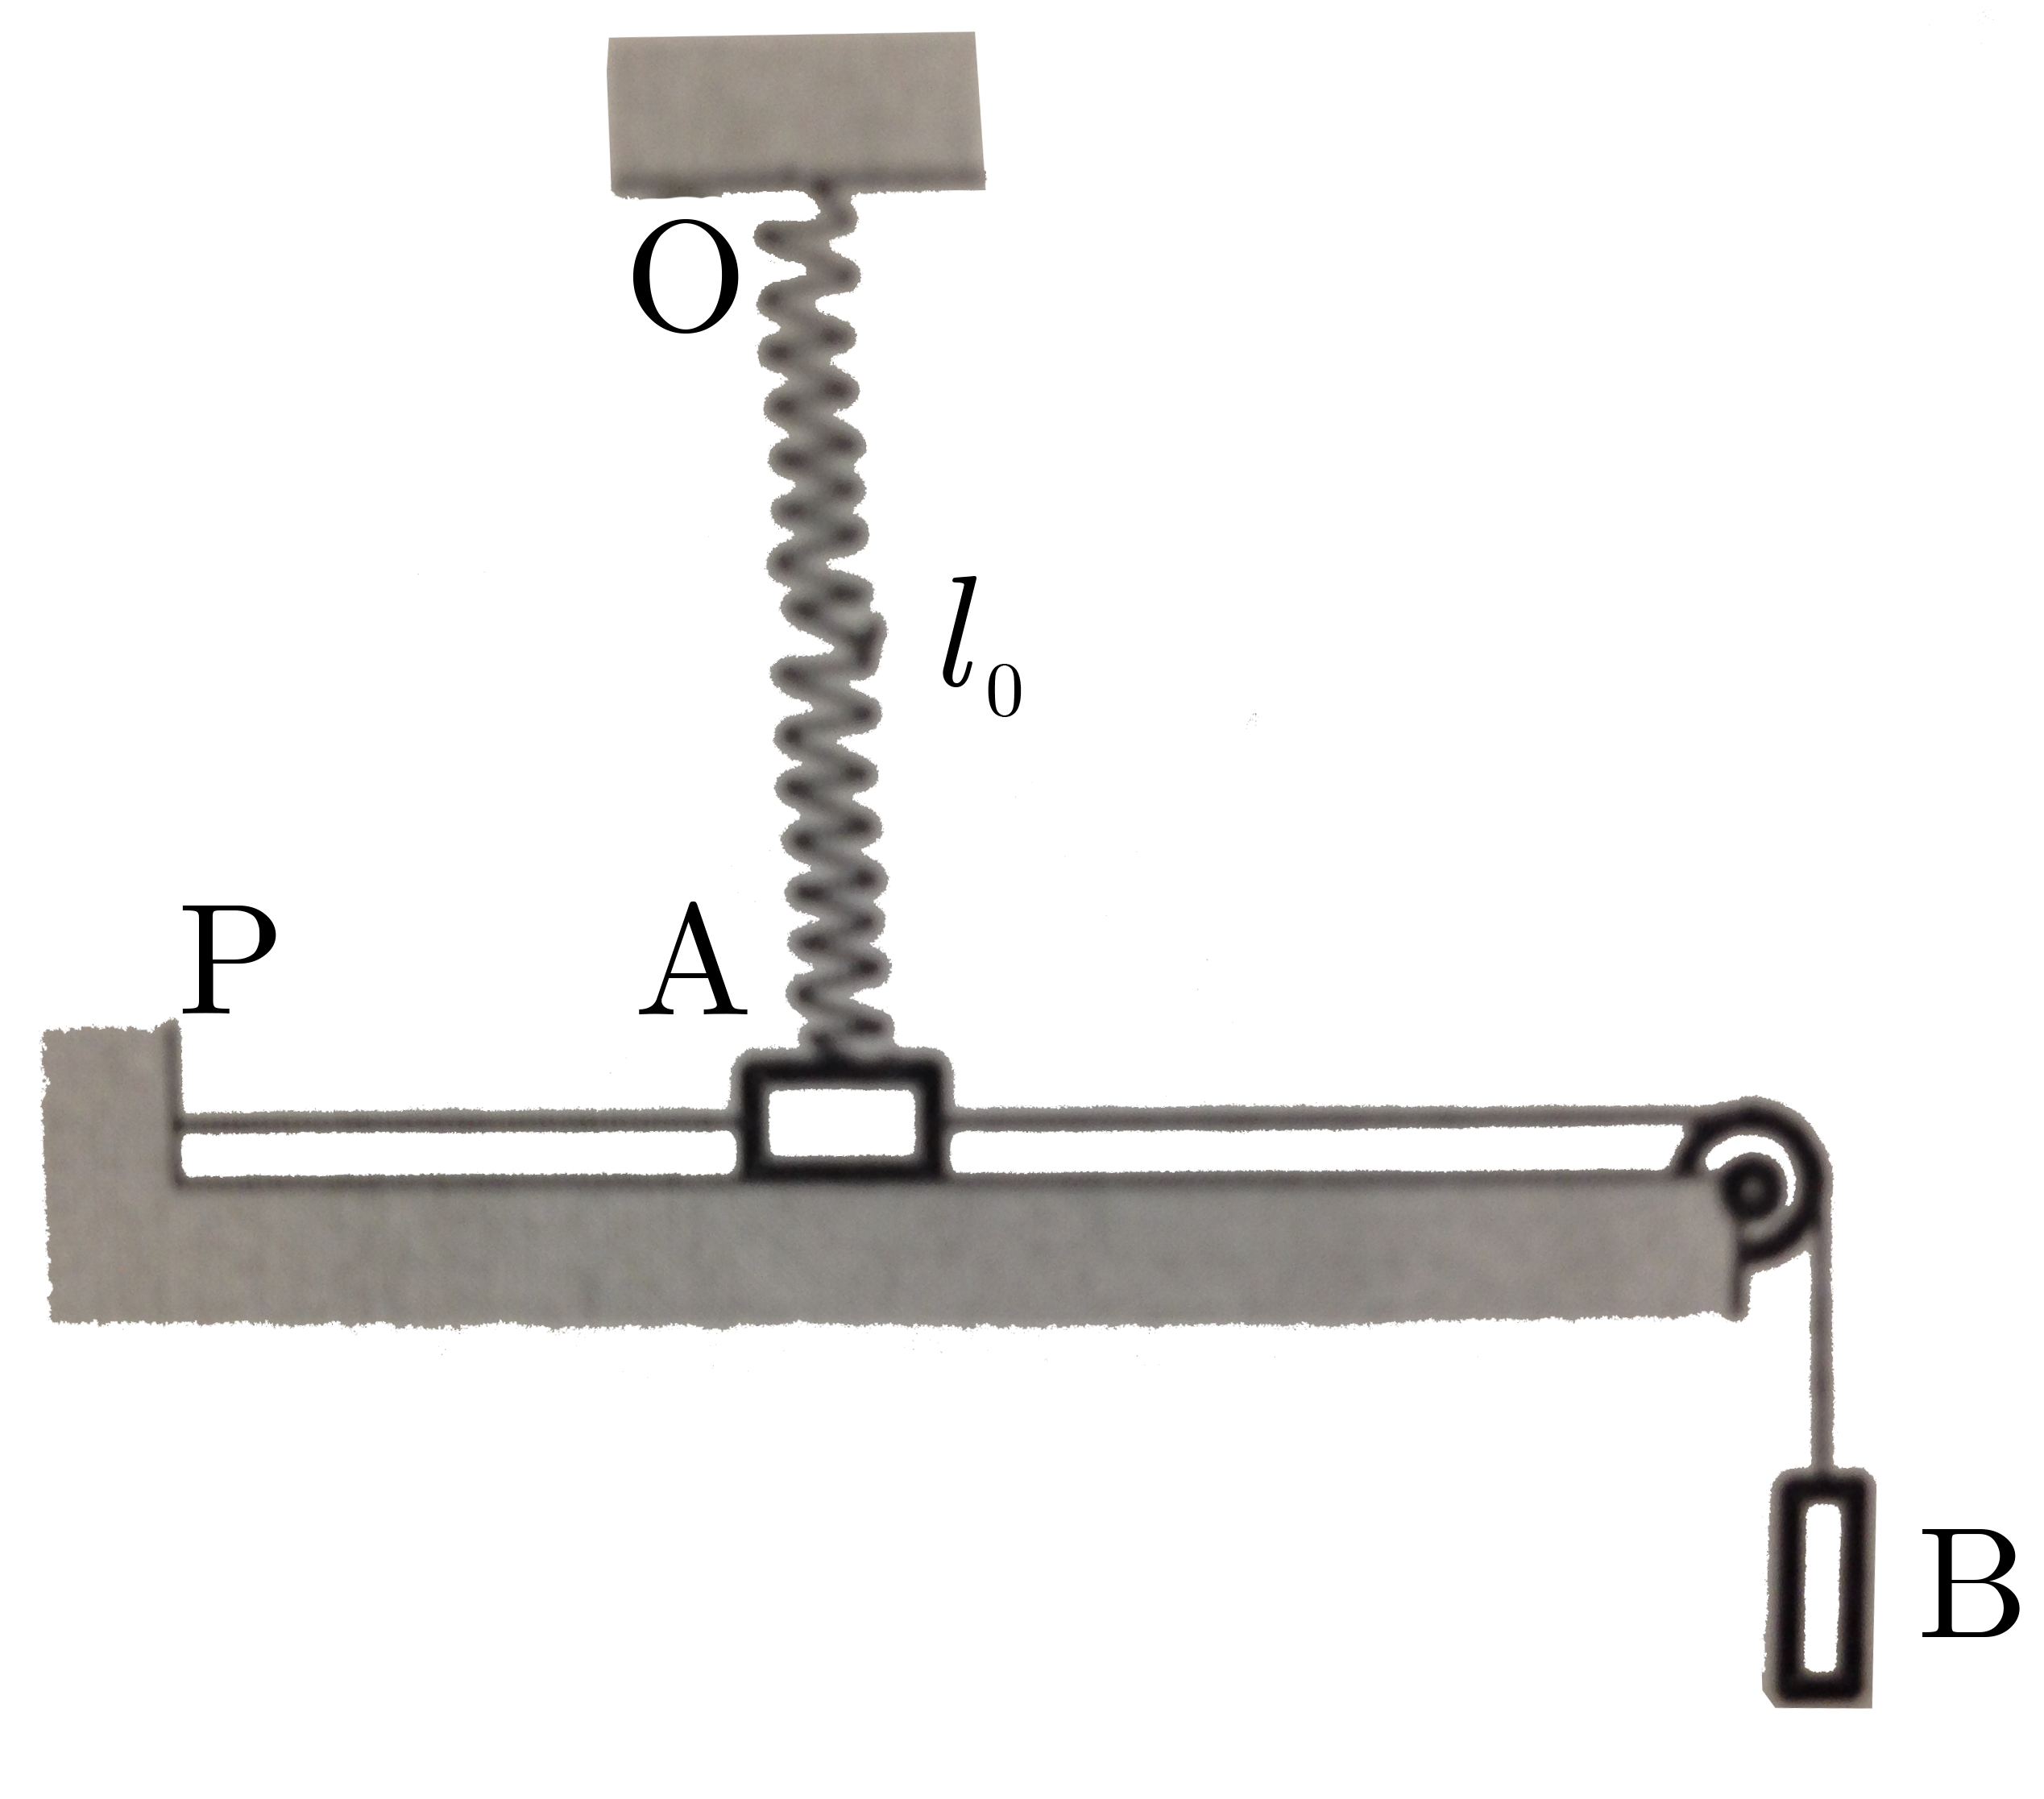
\includegraphics[width=\textwidth]{thread.png}
\end{minipage}
\end{tabular}
\end{enumerate}
\end{document}
